
In this analysis, the charged Higgs boson is decaying to the \PQc and $\bar{\PQs}$ 
quark. The invariant mass of the \PQc$\bar{\PQs}$ system ($\mjj$) is thus used as the 
final observable. The $\mjj$ distribution of two highest \pt, non \PQb jets is
shown in Figures~\ref{subfig:mjj_muBTag} and \ref{subfig:mjj_eleBTag} for
both channels. For the true semileptonic \ttbar events, the mean of the $\mjj$ distribution 
should be close to 80 \GeV, which is the mass of the \PW boson. However, the mean of
$\mjj$, as shown in Figures~\ref{subfig:mjj_muBTag} and \ref{subfig:mjj_eleBTag},
is about 128 \GeV because the two light jets in every event may not necessarily 
come from the decay of a \PW boson. Secondly, the $\mjj$ distribution has a long tail 
which might constrain the search for new resonances in the dijet mode. 
\begin{figure}
    \centering
    \subfigure[With reconstructed jets after \PQb jet selection \label{subfig:mjj_muBTag}]
    {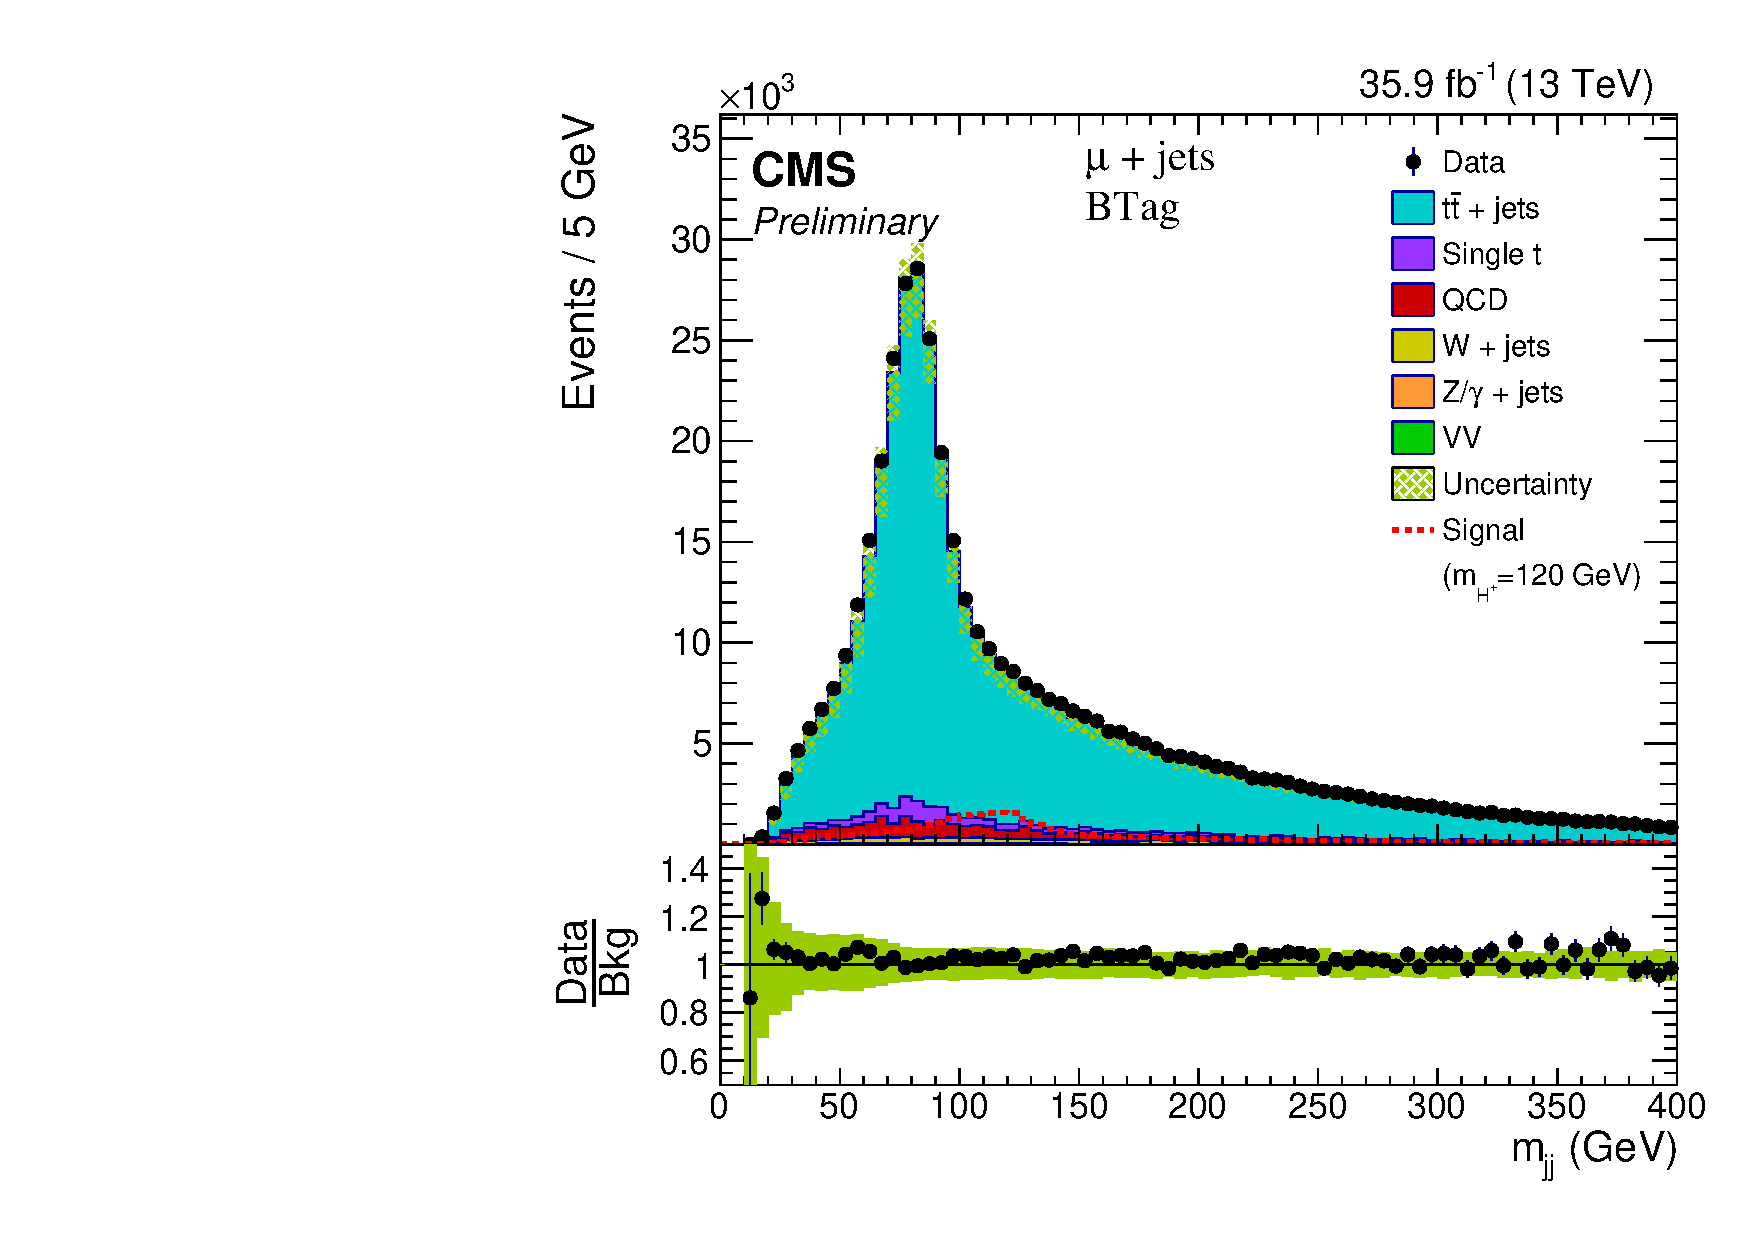
\includegraphics[width=0.49\linewidth]{Image/Muon/BTag/mjj_muBTag.pdf}}
    \subfigure[With reconstructed jets after \PQb jet selection \label{subfig:mjj_eleBTag}]
    {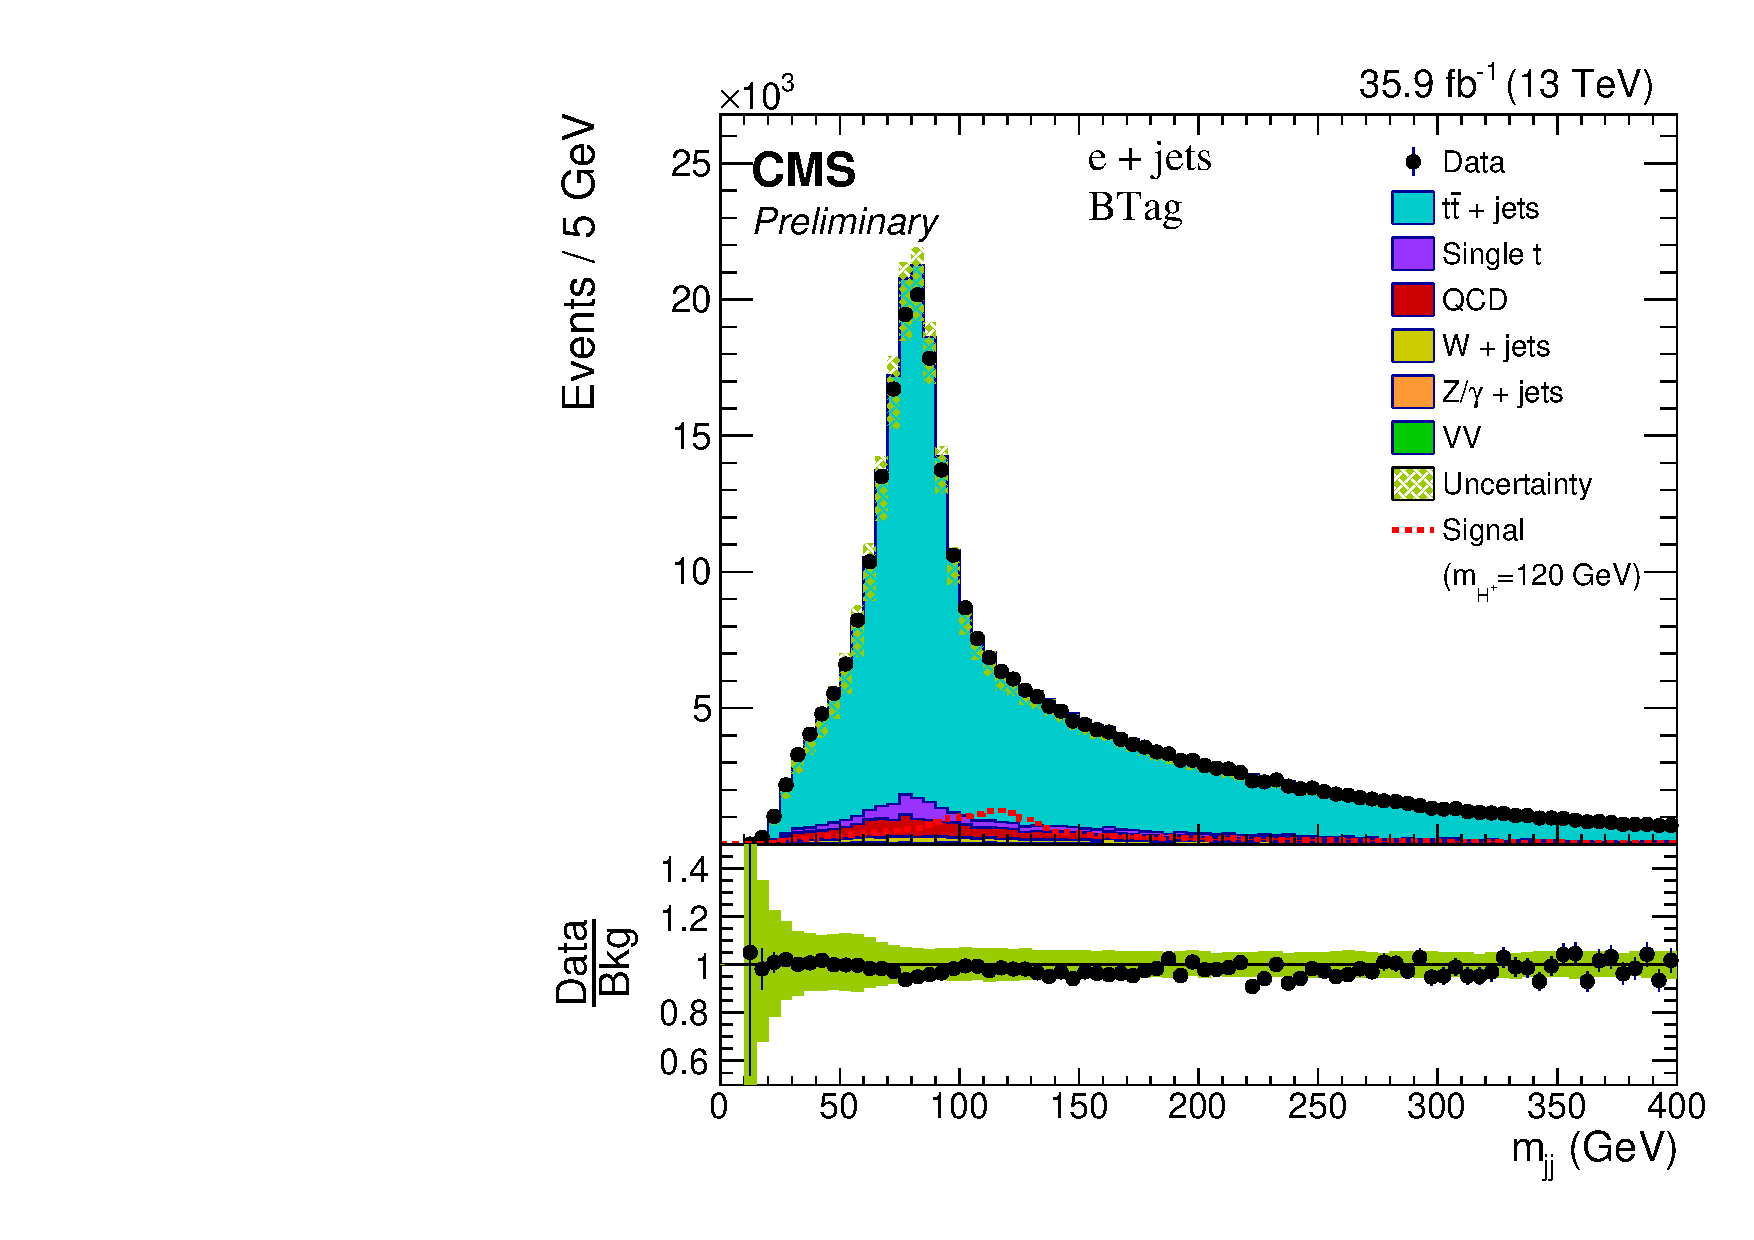
\includegraphics[width=0.49\linewidth]{Image/Electron/BTag/mjj_eleBTag.pdf}}
    \vfil
    \subfigure[With kinematic fitted jets after KF selection \label{subfig:mjj_kfit_muKinFit}]
    {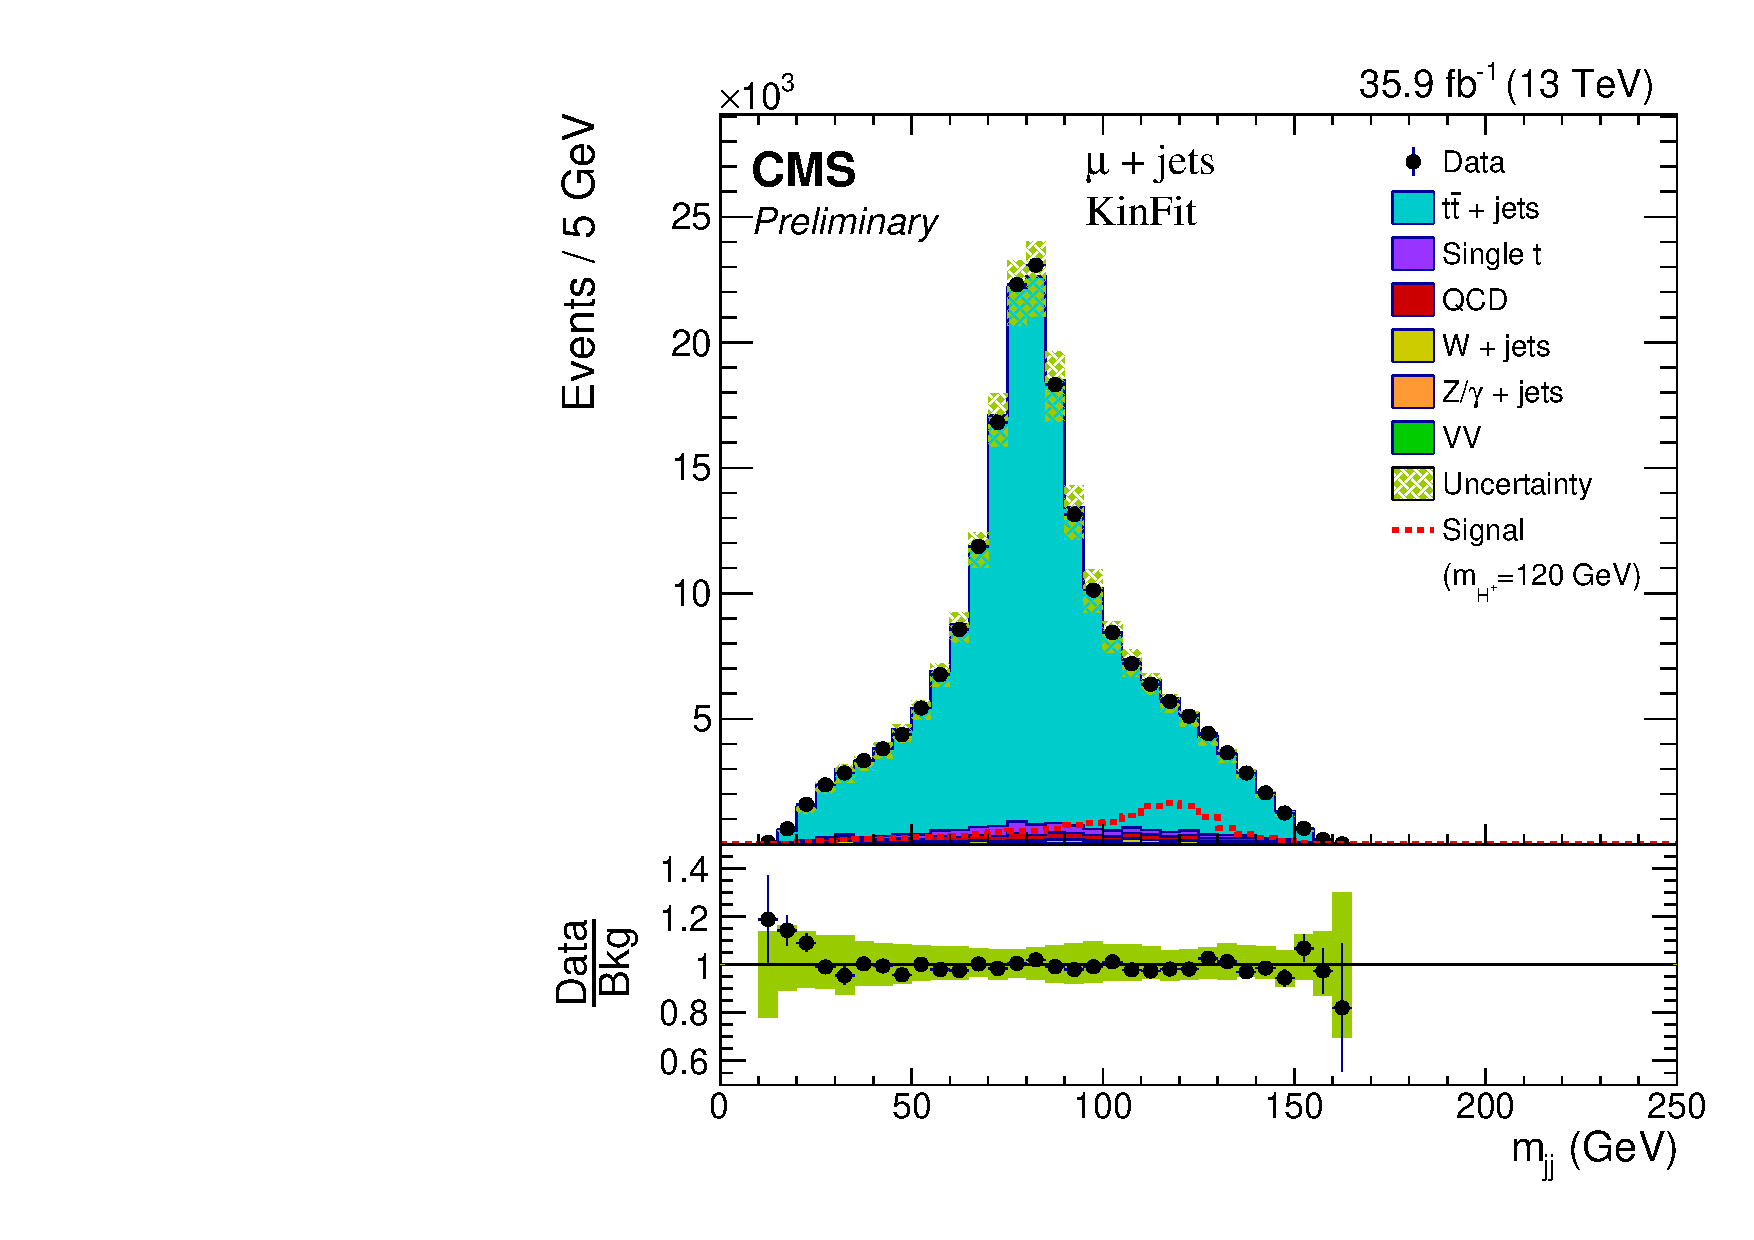
\includegraphics[width=0.49\linewidth]{Image/Muon/KinFit/mjj_kfit_muKinFit.pdf}}
    \subfigure[With kinematic fitted jets after KF selection \label{subfig:mjj_kfit_eleKinFit}]
    {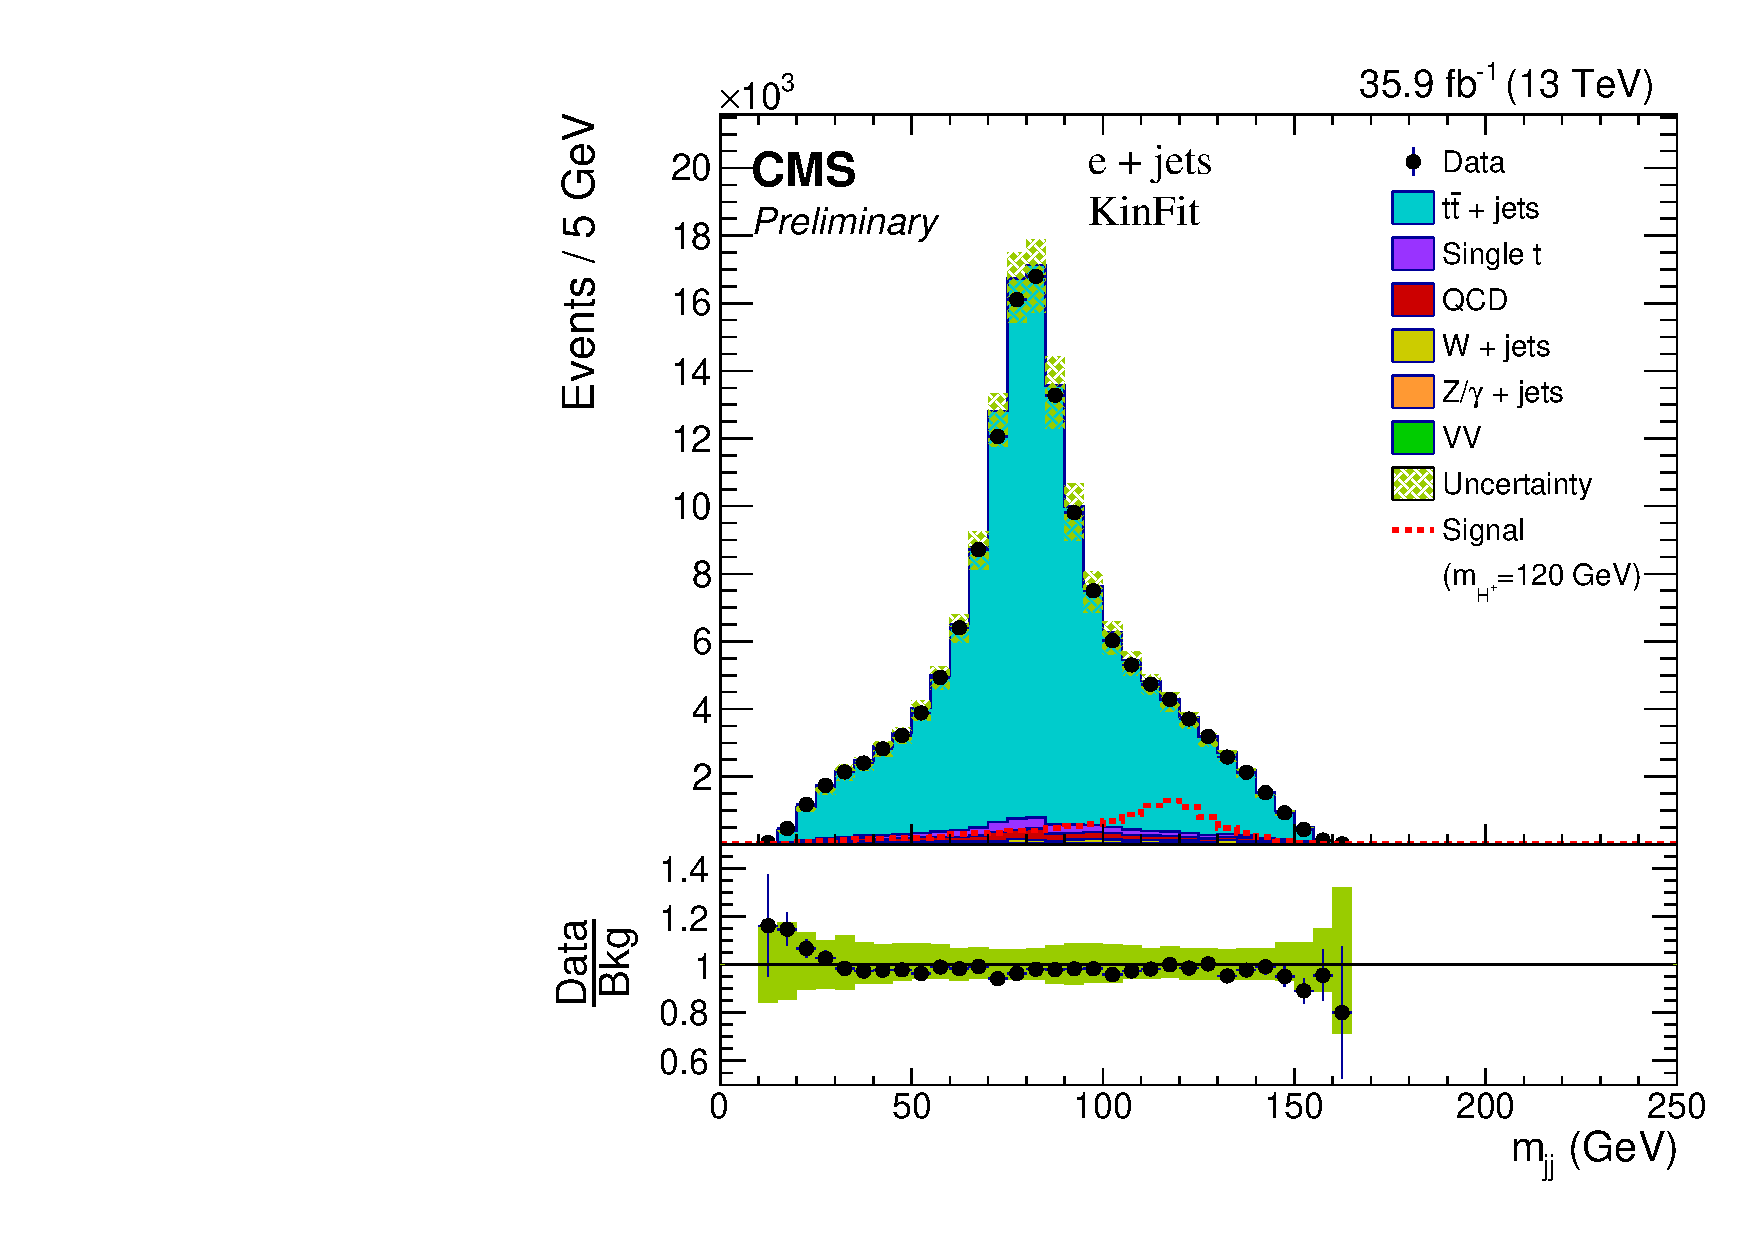
\includegraphics[width=0.49\linewidth]{Image/Electron/KinFit/mjj_kfit_eleKinFit.pdf}}
    \caption{$\mjj$ distributions of two non \PQb, highest \pt jets for the 
     \mujets and \ejets channel. The distributions of 
     Figures~\ref{subfig:mjj_muBTag} and \ref{subfig:mjj_eleBTag} are obtained 
     using reconstructed jets after applying \PQb tag scale factor as described 
     in Section~\ref{s:secEvtSel}. On the other hand, the distributions of 
     Figures~\ref{subfig:mjj_kfit_muKinFit} and \ref{subfig:mjj_kfit_eleKinFit} 
     are calculated using kinematic fitted jets after kinematic fit selection. 
     The mean of the invariant mass distribution from kinematic fitted jets 
     is closer to the \PW mass as compared to that of reconstructed jets.}
    \label{fig:mjjBTagKinFit}
\end{figure}

To select true semileptonic \ttbar events, a kinematic fit is performed on the 
reconstructed objects using the top kinematic fitter package~\cite{DHondt:2006iej}. 
The \verb|TopKinFitter| takes physics objects such as lepton, jets, \MET, and their 
resolutions as input, and gives improved four-vectors of lepton, jets, and neutrino with 
associated $\chi^2$ and probability of the fit as output. It constrains the reconstructed 
\PQt quark mass to its nominal value (\mt = 172.5 \GeV). In the output, the 
\verb|TopKinFitter| gives only four jets (2 \PQb jets from leptonic and hadronic modes, and 2 
light jets from hadronic mode), 1 lepton, and neutrino. It also separates jets coming from
leptonic and hadronic decay modes of \ttbar. The 2 light jets coming from hadronic 
decay mode are further used for \PQc tagging as described in Section~\ref{s:cTag}. 
A more detailed description of the kinematic fitting is given below.

\section{Input to the TopKinFitter}
\label{ss:inputKF} 
After applying selection criteria on physics objects as described
in Section~\ref{s:secEvtSel}, the event which is passed to the \verb|TopKinFitter| contains 
only one lepton, \MET and at least 4 jets. The \PQb discriminator value with the medium 
working point is also given as the input to the \verb|TopKinFitter| to separate \PQb jet 
from light jets (more details in Section~\ref{ss:jetSepKF}). The constraints on the \ttbar 
system along with the theoretical mass of the \PQt quark are also specified
(more details in Section~\ref{ss:constraintKF}). All the constraints and invariant mass are 
parameterized in terms of $E_{T}$, $\eta$, and $\phi$ variables of the physics objects. 
The components of 4-momentum vector in terms of these variables are given as
\begin{equation}
E = E_{T} \sin\theta, p_x = E_{T}\cos\phi, p_y = E_{T}\sin\phi, p_z = E_{T}\cot\theta,
\end{equation}
and the invariant mass of two particles, in the relativistic limit, is given by
\begin{equation}
	m_{\rm{inv}} = \sqrt{2 E_{T_1}E_{T_2}\left(\cosh(\eta_1 - \eta_2) - \cos(\phi_1 - \phi_2)\right)}
\end{equation}
where $\eta = \ln\cot(\theta/2)$. The resolution of each physics object as a function of 
\pt and $\eta$, and the JER scale factors from different $\eta$ binning are also given in the 
input. Apart from the physics objects, various inputs related to the minimization of 
$\chi^2$ such as the maximum number of iterations, criteria on the convergence of the $\chi^2$
are also specified (more details in Section~\ref{ss:chi2KF}).

\section{Separation of jets}
\label{ss:jetSepKF} 
For the semileptonic decay mode of the \ttbar, the first step is to separate 2 
\PQb jets from light jets and the second step is to identify each \PQb jet from hadronic 
and leptonic modes.  All the jets are sorted in their \pt order and first 4 jets are
selected. To find out the two \PQb jets, a \PQb tag probability is calculated using 
following formula \cite{DHondt:2006iej}
\begin{equation}
	L_{b}(x) = \frac{\text{PDF}_b(x)}{\sum_{i=1}^5 \text{PDF}_i(x)}
\end{equation}
Where $\text{PDF}_i(x)$ is the probability distribution function of \PQb discriminator value
(x) for flavour $i$. An event is selected if two jets have \PQb tag probability of more 
than 60\%. The jet-parton matching is also performed for each jet. For n number of 
jets, there are exactly n number of partons. The number of permutations in the 
jet-parton matching is given by
\begin{equation}
	N_{\rm{permutations}} = \frac{n!}{(n-4)!}
\end{equation}
Therefore for 4 jets, there are 24 permutations. All the 24 permutations are shown 
in \cite{KinFitThesis} through diagrams. However, after identifying two \PQb jets, the number of 
permutations reduces to 12 as the two \PQb jets are interchangeable. For each 
jet-parton permutation, a $\chi^2$ is constructed, as described in Section
\ref{ss:chi2KF}, and the permutation with the lowest value of $\chi^2$ is
treated as the correct matching. Afterward, three jets (1 \PQb jet and 2 light jets) 
have to be selected to form hadronic decaying \PQt quark. For this, several sensitive 
variables are used \cite{DHondt:2006iej} such as the angle between jets and lepton, 
angular separation between the generated and reconstructed jets, etc.

\section{Kinematic constraints}
\label{ss:constraintKF} 
The semileptonic decay mode of the \ttbar has 4 jets, 1 lepton and the neutrino in 
the final state. The x and y-component of the neutrino are taken from the \MET, as the 
missing transverse energy is attributed to the neutrino. And the z-component of the 
neutrino, $p^v_z$, is determined from the fit. The following kinematic constraints are 
imposed on the semileptonic \ttbar system
\begin{subequations}
\begin{eqnarray}
	m_{\rm{inv}}(b^{\text{had}}q\bar{q}) = m_{t} = 172.5 \text{\GeV} \label{eq:constraintKF1}\\
	m_{\rm{inv}}(b^{\text{lep}}l\nu_l)   = m_{\bar{t}} = 172.5 \text{\GeV} \label{eq:constraintKF2}
\end{eqnarray}
\label{eq:constraintKF}
\end{subequations}
After the fit, the $p^v_z$ is determined from the Equation (\ref{eq:constraintKF2}). 
For every event, a $\chi^2$ is constructed as discussed in Section~\ref{ss:chi2KF}.
The $\chi^2$ is minimized by varying \pt, $\eta$, and $\phi$ of each object within
their resolution. Those values of \pt, $\eta$, and $\phi$ variables are finally selected 
which minimises the $\chi^2$ and at the same time satisfies Equation (\ref{eq:constraintKF}).

\section{$\chi^2$ of the fit}
\label{ss:chi2KF} 
For every selected event, a $\chi^2$ is constructed which is given by
\begin{equation}
	\chi^2 = \left(\frac{m_t - 172.5}{\sigma_{m_{t}}}\right)^2 + 
	\left(\frac{m_{\bar{t}} - 172.5}{\sigma_{m_{\bar{t}}}}\right)^2+
	\sum_{i}\left(\frac{p_i^{\text{fit, lep}} - p_i^{\text{lep}}}{\sigma_{p^{\text{lep}}_i}}\right)^2+
	\sum_{j}\sum_{i}\left(\frac{p_i^{\text{fit}, \text{jet}_j} - 
	p_i^{\text{jet}_j}}{\sigma_{p^{\text{jet}_j}_i}}\right)^2
\label{eq:chi2KF}
\end{equation}
where $\sigma_{m_{t}}$ is the resolution of the mass of the \PQt quark and $\sigma_{p_{i}}$ 
is the momentum resolution of three component ($i= 1, 2, 3$) of the corresponding lepton and jets.
The $p^{\text{fit}}$ is the fitted momentum of the given lepton and jets. The $\chi^2$, given in 
Equation (\ref{eq:chi2KF}), is minimized using the Lagrangian multipliers under the constraints 
given in Equation (\ref{eq:constraintKF}). A detailed mathematical description for the minimization 
of the $\chi^2$ is given in \cite{DHondt:2006iej}. The $\chi^2$ is minimized iteratively where in 
each step the 4 components of the momentum vector of each object are varied
within their resolution and a $\chi^2$ and the constraint is calculated. The
fit is declared to be converged if the following constraints are satisfied
\begin{subequations}
\begin{eqnarray}
	\frac{\chi^2 (n-1) - \chi^2 (n)}{\text{ndf}} < \epsilon_{\chi}\\ 
	m_{\rm{inv}}(b^{\text{had}}q\bar{q}) - 172.5 < \epsilon_{c}\\
        m_{\rm{inv}}(b^{\text{lep}}l\nu_l) - 172.5 < \epsilon_{c}
\end{eqnarray}
\end{subequations}
where $\epsilon_{\chi} = 5\times 10^{-05}$, $\epsilon_{c} = 0.0001$, and \text{ndf}
is the number of degrees of freedom which is equal to 1 as we have two 
constraints and one free parameter ($p_z^\nu$). The total number of iterations ($n$)
is 500.

\section{Output of the TopKinFitter}
\label{ss:outputKF} 
For every event, the \verb|TopKinFitter| gives the status of fit which is 0 if 
the fit converged and 1 if it did not, $\chi^2$ of the fit, probability ($P_{\chi}$) 
of the goodness-of-fit of $\chi^2$, and the 4 momentum vector of physics objects such
as jets, lepton and a neutrino. The $\chi^2$ and $P_{\chi}$ are related by the 
following equation
\begin{equation}
	P_{\chi} = \exp(\frac{-\chi^2}{2})
\end{equation}
The fit also separates jets from hadronic and leptonic decay mode of \ttbar, 
that is, it gives one hadronic \PQb jet, one leptonic \PQb jet, and 2 light jets from hadronic
decay modes. The \PQc tagging criteria are applied further on the 2 light jets as 
discussed in Section \ref{s:cTag}. The $\mjj$ distribution of the light jets is used in 
further analysis.

\section{Selection and performance}
\label{ss:selKF} 
Due to wrong jet combinatorics, the fit does not converge for every event. Only 
those events are selected for which the fit converges. The efficiency of fit convergence 
is 73\% for simulated \ttbar sample and 71\% for data for both channels.
Further, the angular separation between reconstructed and kinematic fitted 
lepton and jets are required to be less than 0.2 to make sure that they are almost in the same
direction. The same $\Delta \rm R$ cut is applied on reconstructed and kinematic
fitted jets. Also, the \pt cut on kinematic fitted lepton and jets are required to
be the same as that on the reconstructed jets and lepton. After applying these additional 
cuts on $\Delta \rm R$ and \pt, the kinematic fit efficiency reduces to 47\% for \ttbar 
and 44\% for data for both channels. In summary, the following kinematic fit selections are applied: 
\begin{itemize}[leftmargin=*]
 \item fit is converged,
 \item $\Delta \rm R (\text{fitted lepton, reconstructed lepton}) < 0.2$,
 \item $\Delta \rm R (\text{fitted jet, reconstructed jet}) < 0.2$%, and
% \item $\chi^2_{kfit} >0$, $Prob_{kfit} > 0$.
\end{itemize}
Event yields after kinematic fit selections are shown in the 7th column of Tables~\ref{tab:cutflow_mu},
\ref{tab:cutflow_ele}, \ref{tab:cutflow_mu_sig} and \ref{tab:cutflow_ele_sig}.
From these tables, we see that almost half the number of events is reduced after these selections. 
The $\mjj$ distribution from the two light jets after kinematic fit selection is shown in 
Figures~\ref{subfig:mjj_kfit_muKinFit} and \ref{subfig:mjj_kfit_eleKinFit} for both channels. 
The mean of these distributions is 84\GeV which is close to the mass of \PW boson. 

The kinematic fit is also performed after applying jet energy corrections such as JES and JER.
For up and down systematics of JES and JER, the fit is performed separately 
on every event after correcting jet \pt using the corresponding scale factors.
The output of the fit for each systematic is stored in a different collection
using the \verb|EDProducer|. The kinematic fitting is a time-consuming process 
which takes, on average 0.002 seconds per event for \ttbar process. Therefore, 
performing all (nominal, \verb|JESup|, \verb|JESdown|, \verb|JERup|, and 
\verb|JERdown|) the kinematic fitting takes a reasonable amount of time.

\section{Comparison of data and background after kinematic fitting}
\label{s:secCPlotsKF}

Data to background comparison of variables from the kinematic fitted objects after kinematic 
fit selection are shown in Figures~\ref{fig:kfitPlot1},~\ref{fig:kfitPlot2}, and~\ref{fig:kfitPlot3}. 
There is also a good agreement between data and simulation within the statistical and systematic 
uncertainties. Here also we see a similar disagreement for the higher value of \pt and \MET as
we have after \PQb jet selection described in Section~\ref{s:secEvtSel}.

%After KinFit: Pt_lep, Eta_lep, Pt_jets
\begin{figure}
    \centering  
    \subfigure[\pt of muon]{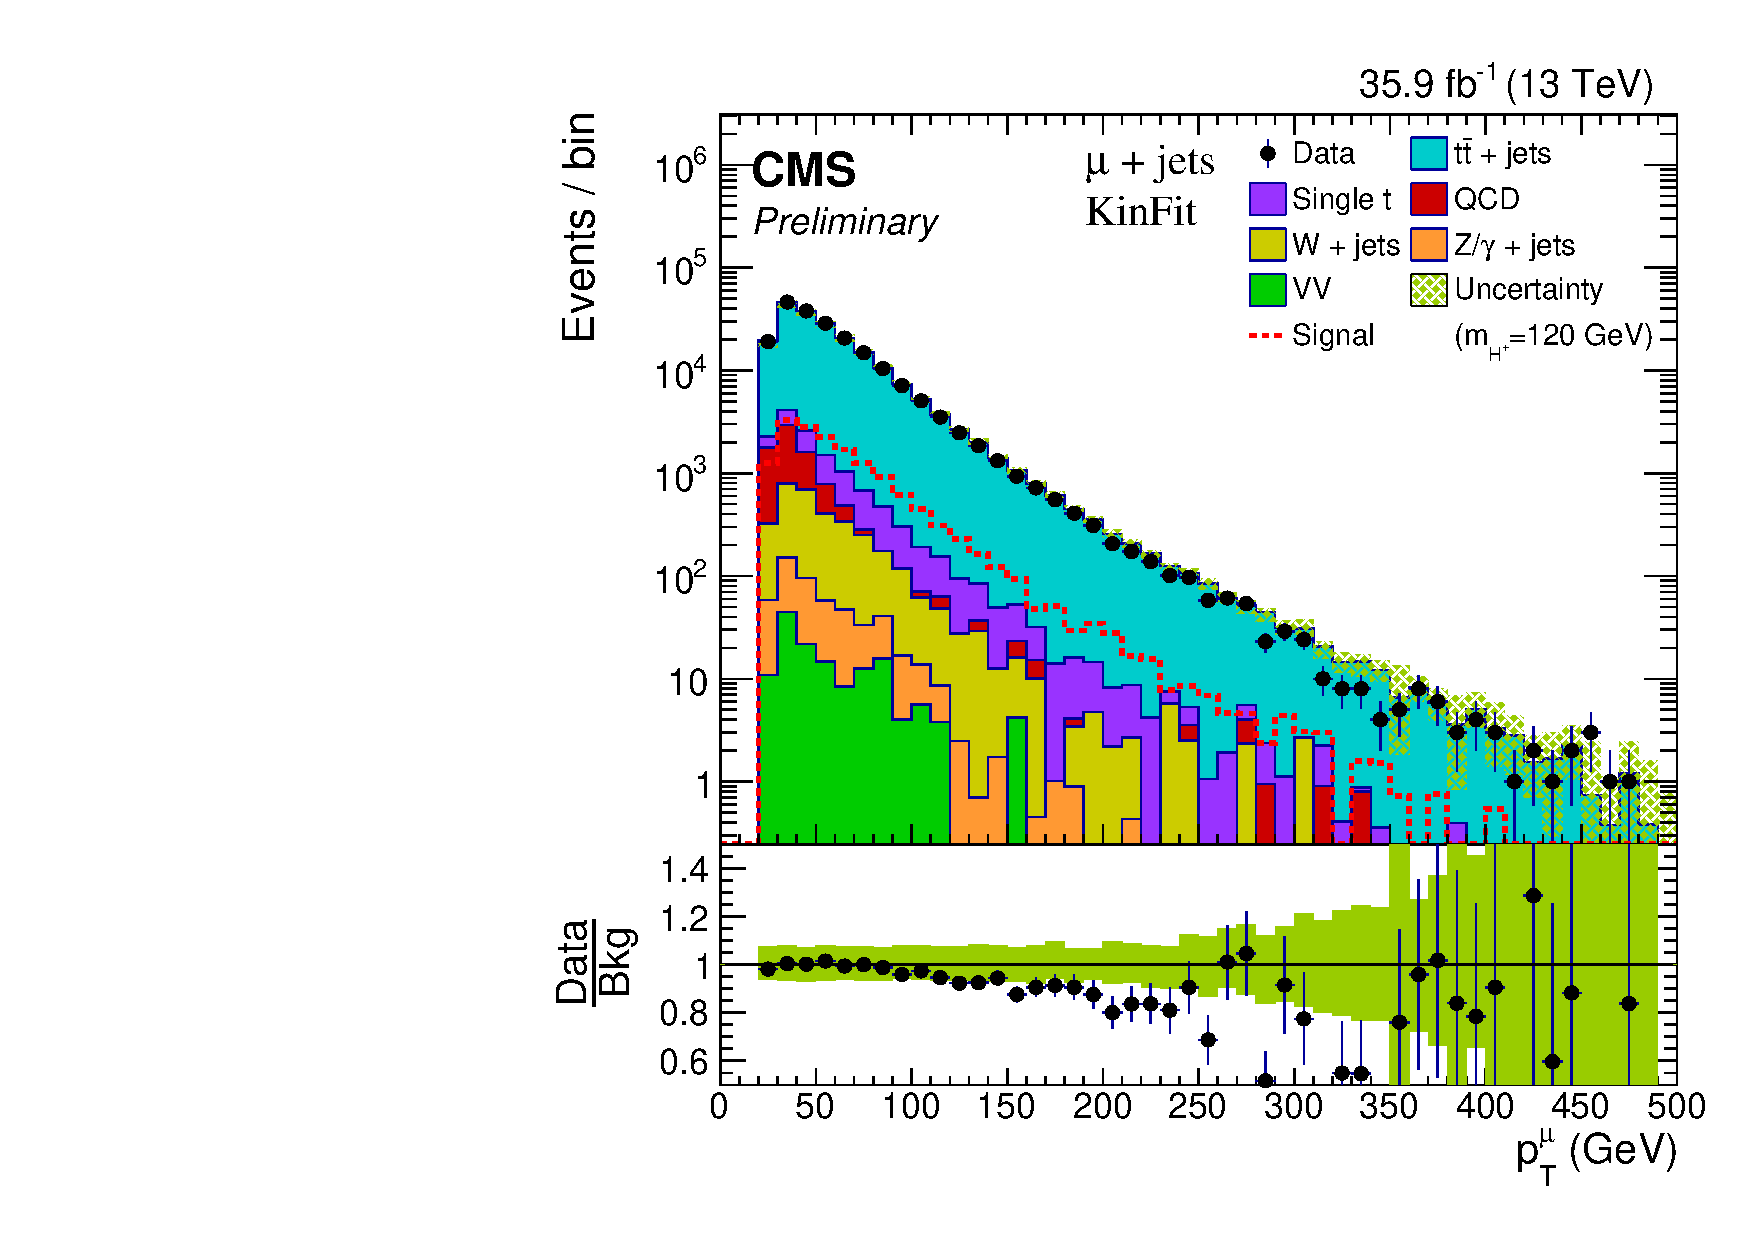
\includegraphics[width=0.40\linewidth]{Image/Muon/KinFit/pt_mu_muKinFit.pdf}}
    \subfigure[\pt of electron]{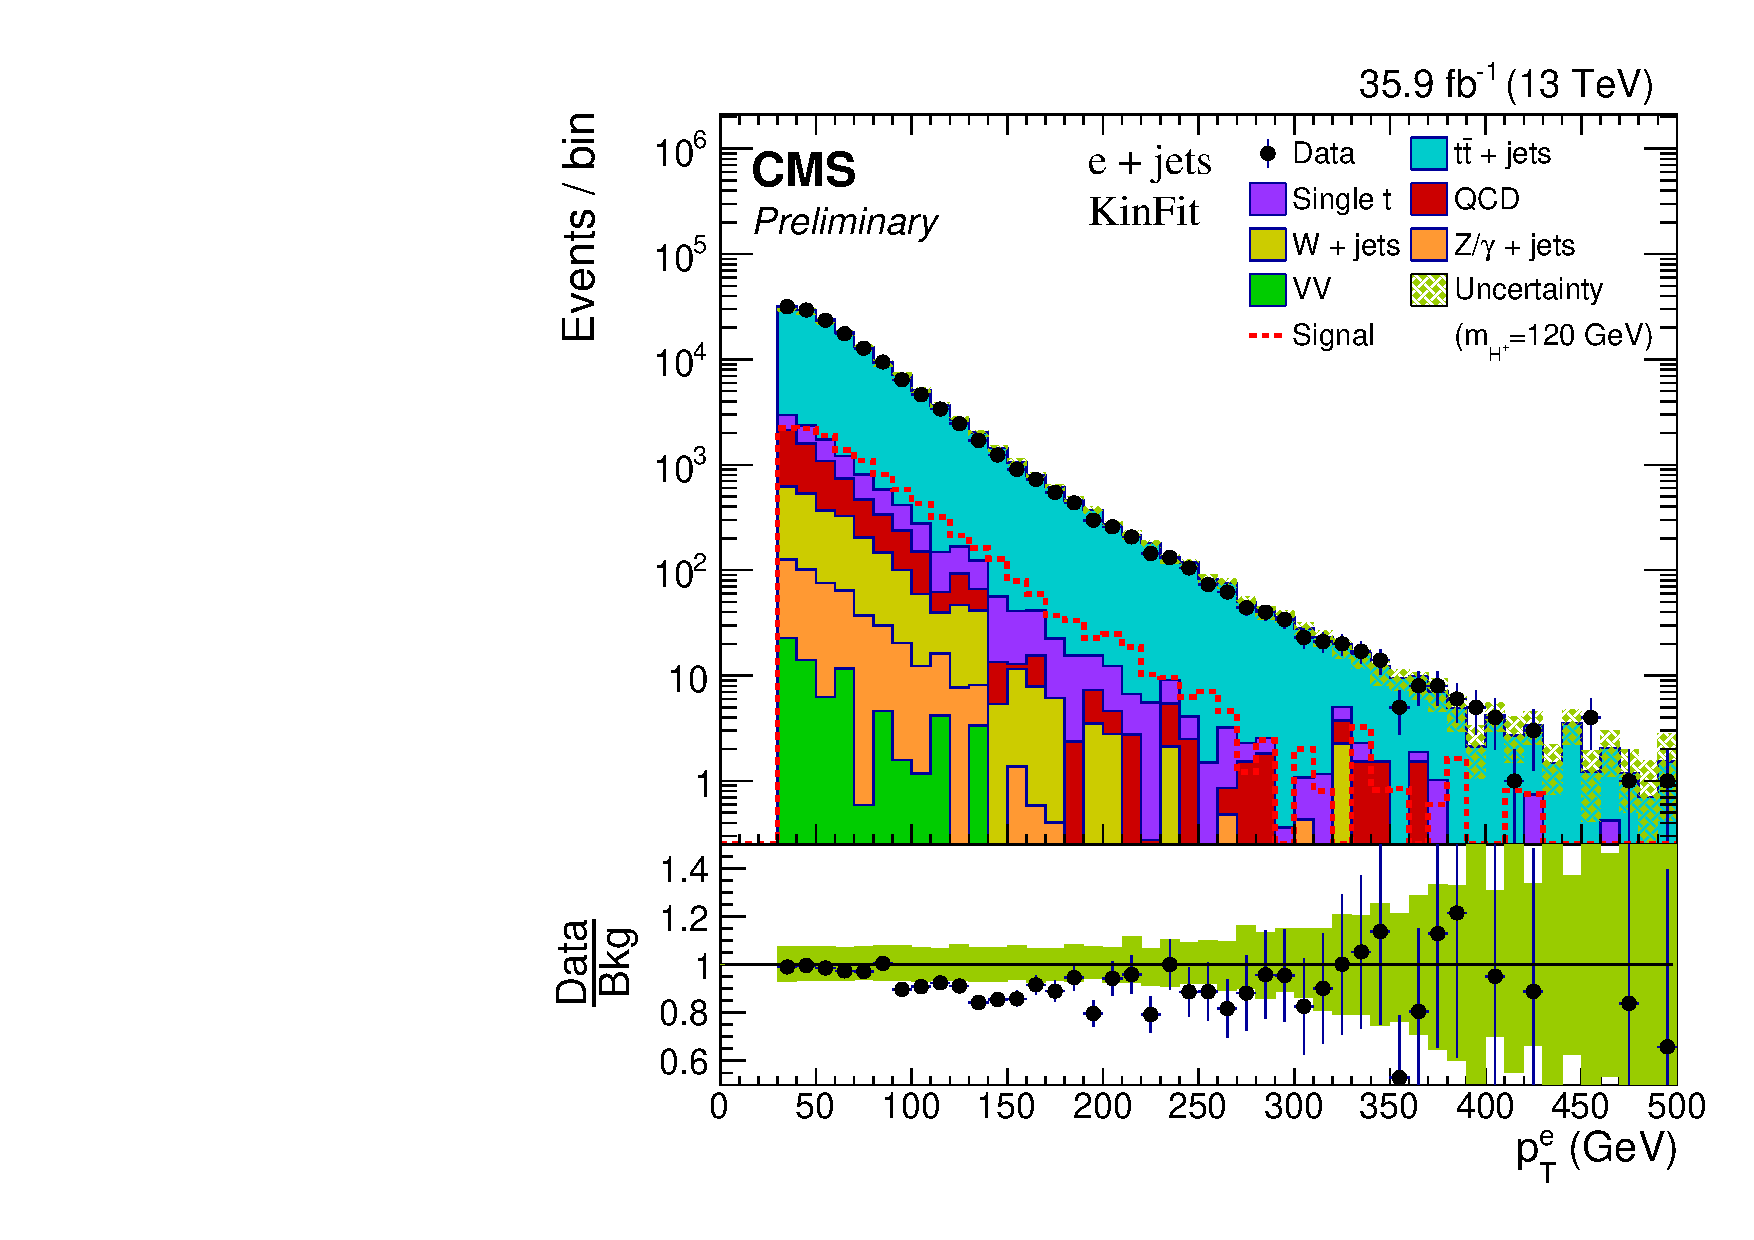
\includegraphics[width=0.40\linewidth]{Image/Electron/KinFit/pt_ele_eleKinFit.pdf}}
    \vfil
    \subfigure[$\eta$ of muon]{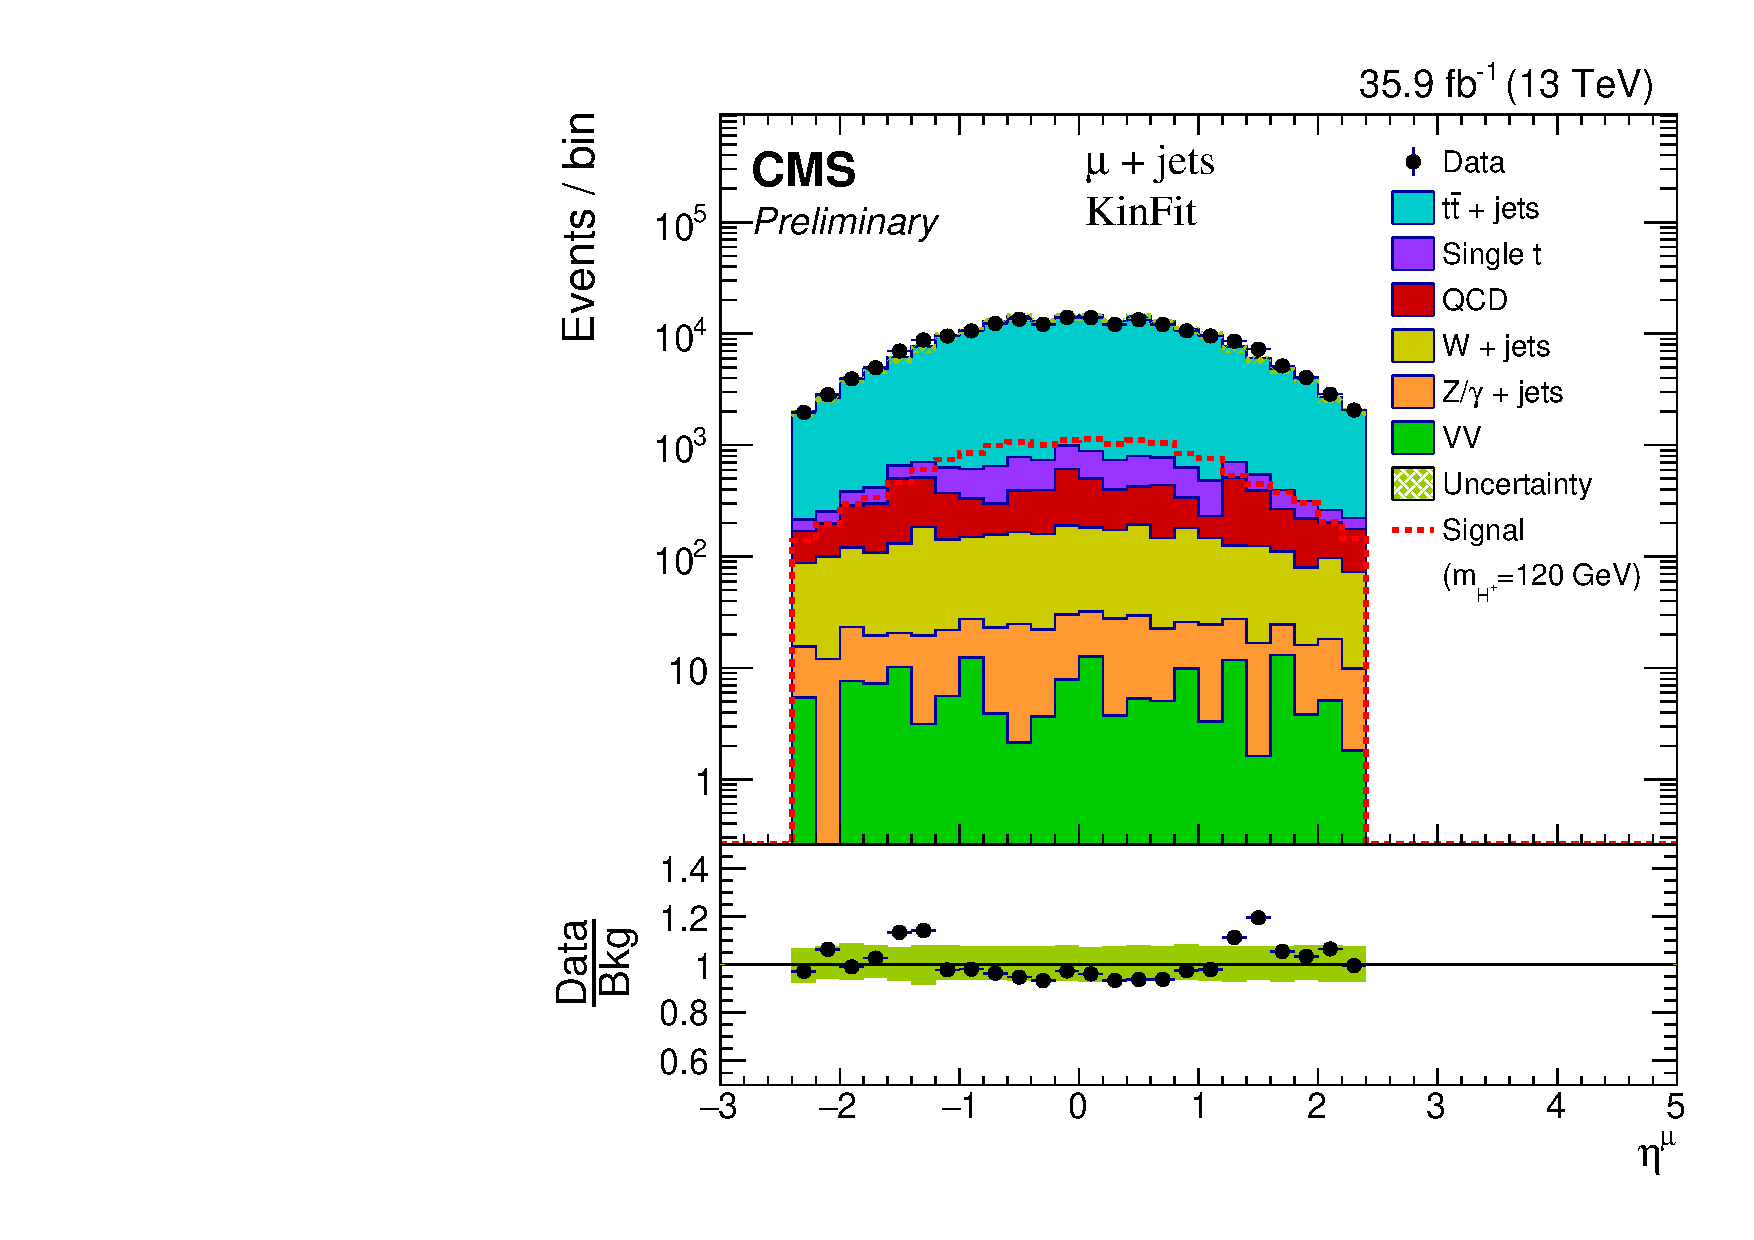
\includegraphics[width=0.40\linewidth]{Image/Muon/KinFit/eta_mu_muKinFit.pdf}}
    \subfigure[$\eta$ of electron]{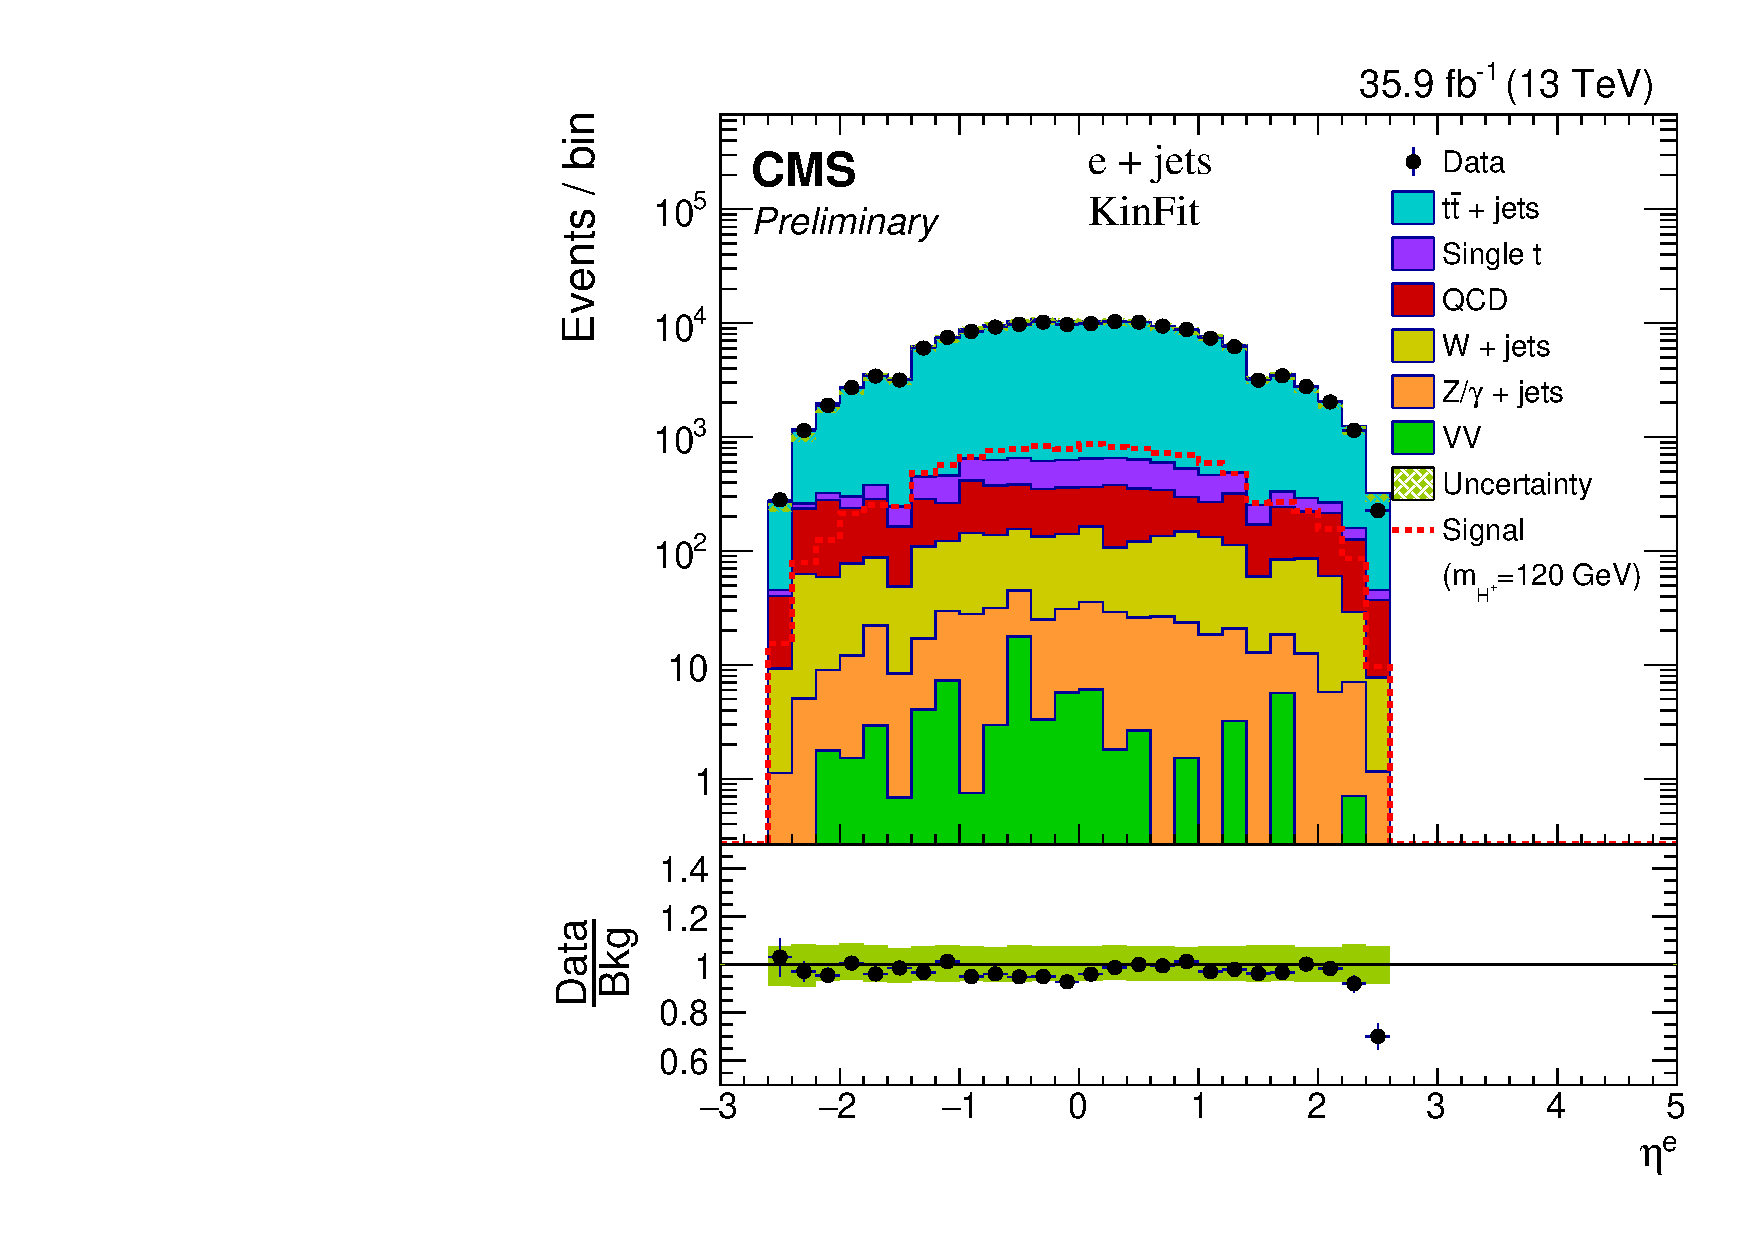
\includegraphics[width=0.40\linewidth]{Image/Electron/KinFit/eta_ele_eleKinFit.pdf}}
    \vfil
    \subfigure[\pt of jets]{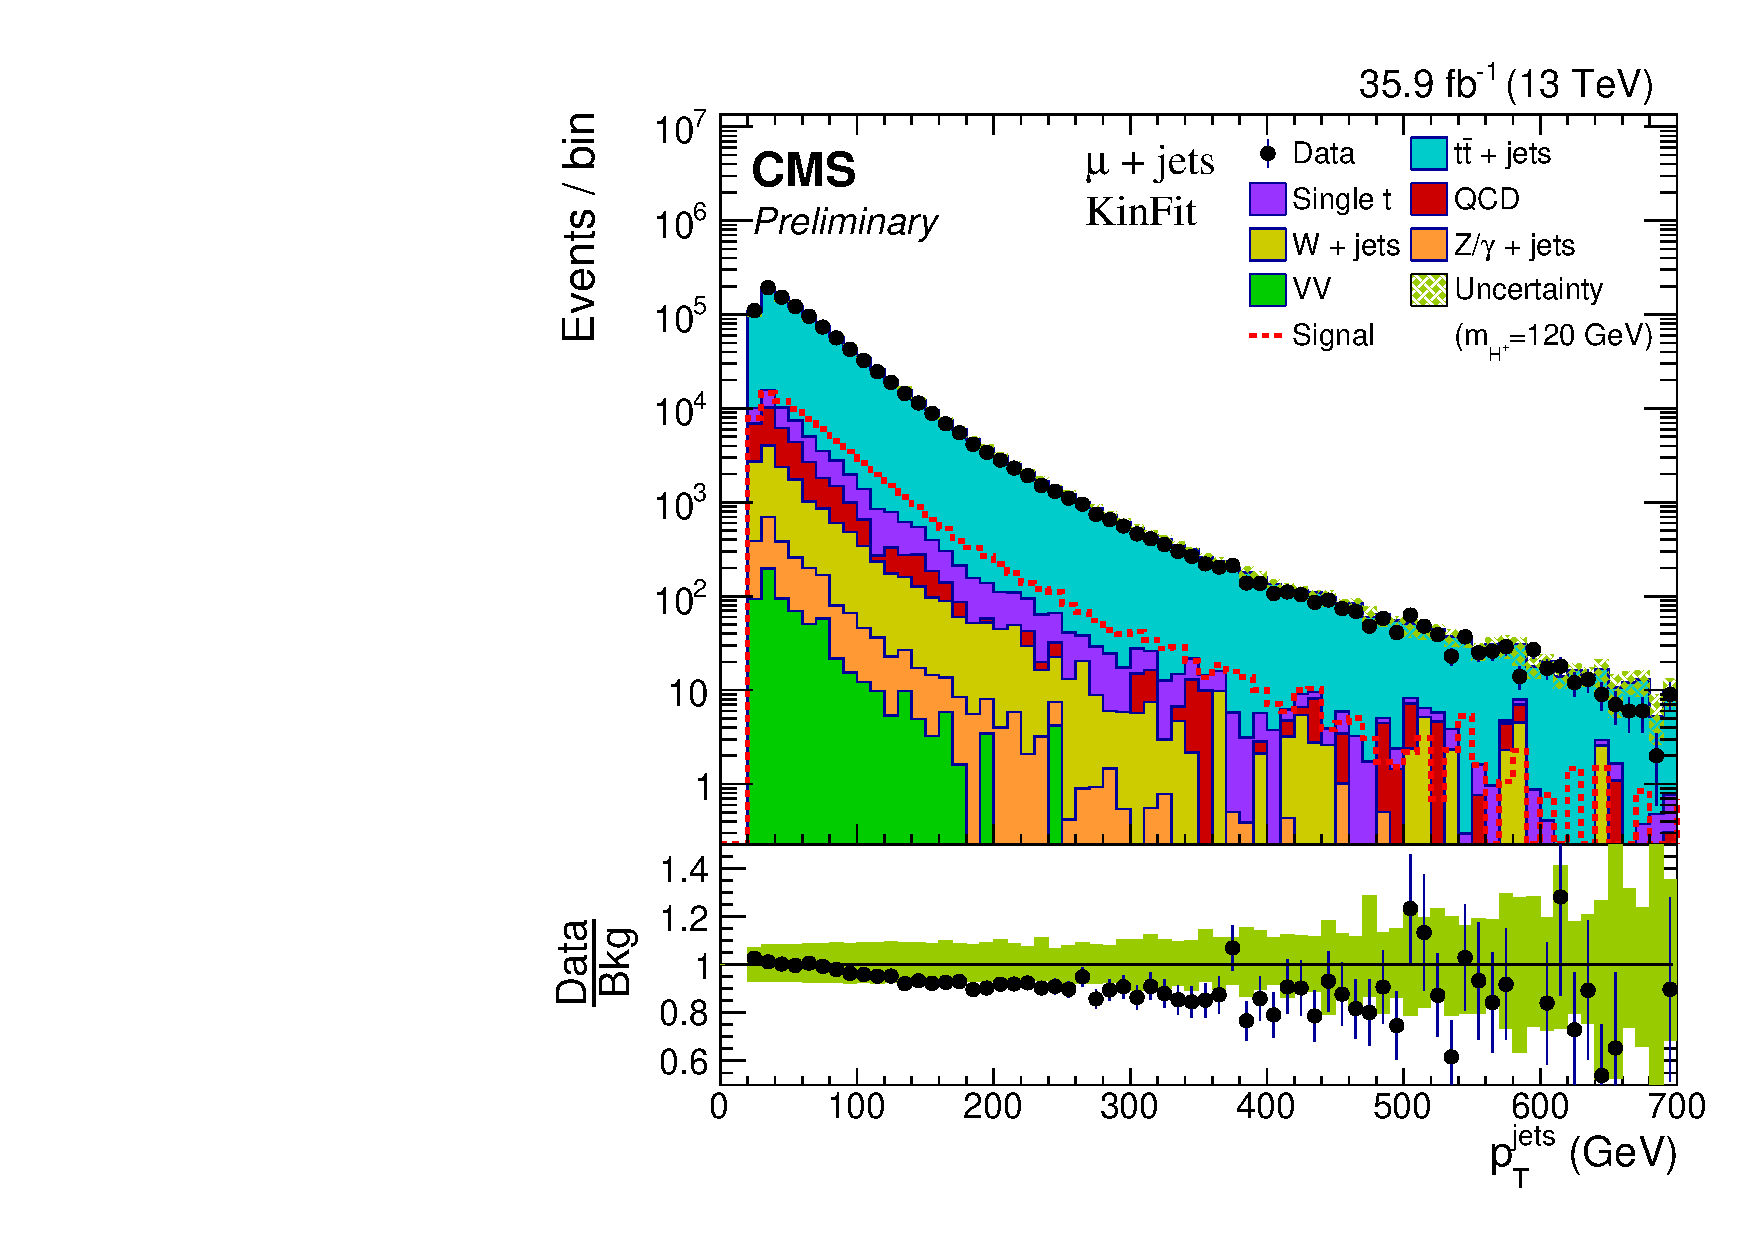
\includegraphics[width=0.40\linewidth]{Image/Muon/KinFit/pt_jet_muKinFit.pdf}}
    \subfigure[\pt of jets]{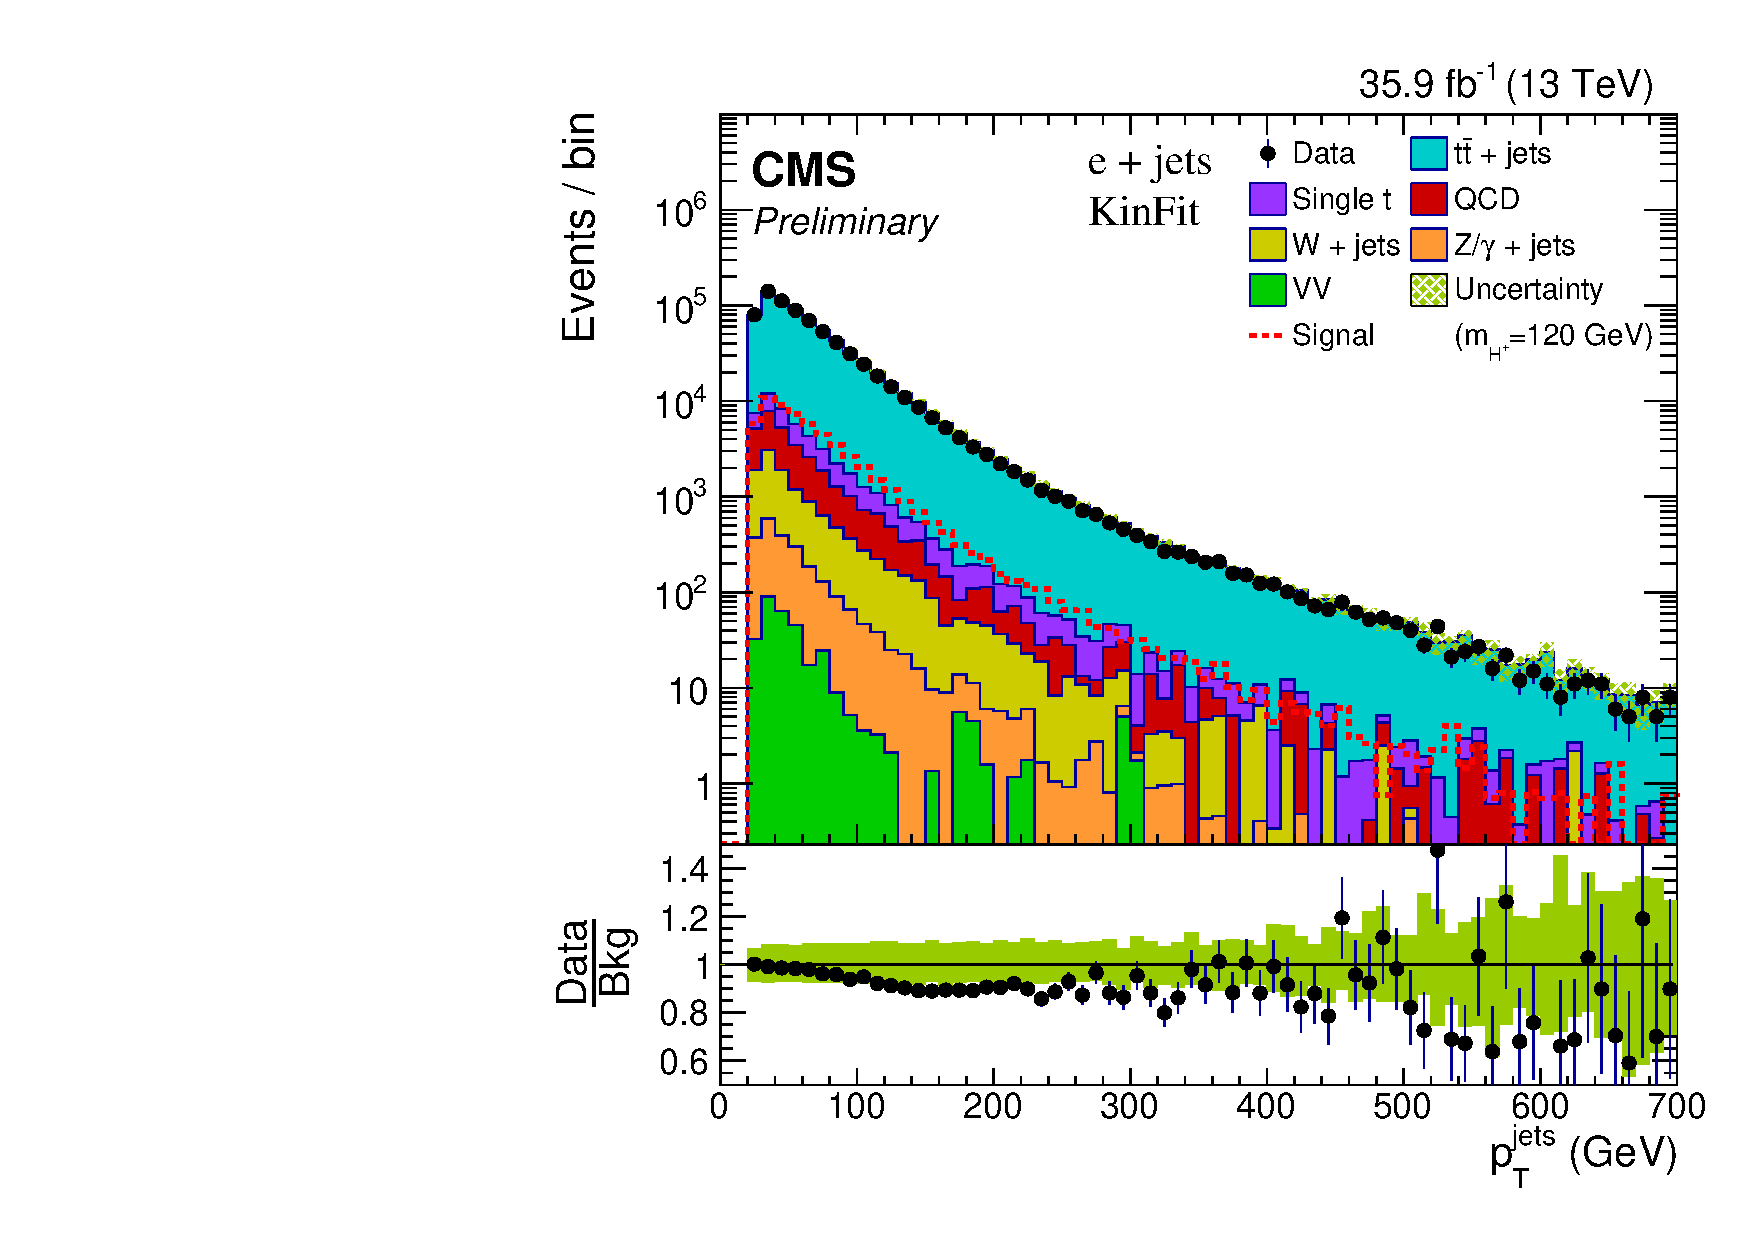
\includegraphics[width=0.40\linewidth]{Image/Electron/KinFit/pt_jet_eleKinFit.pdf}}
    \caption{Distribution of $\pt, \eta$ of kinematic fitted lepton and $\pt$ of jets
    after kinematic fit selection for \mujets and \ejets channel.}
    \label{fig:kfitPlot1}
\end{figure}

%After KinFit:Eta_jets , N_jets, N_bjets
\begin{figure}
    \centering  
    \subfigure[$\eta$ of jets]{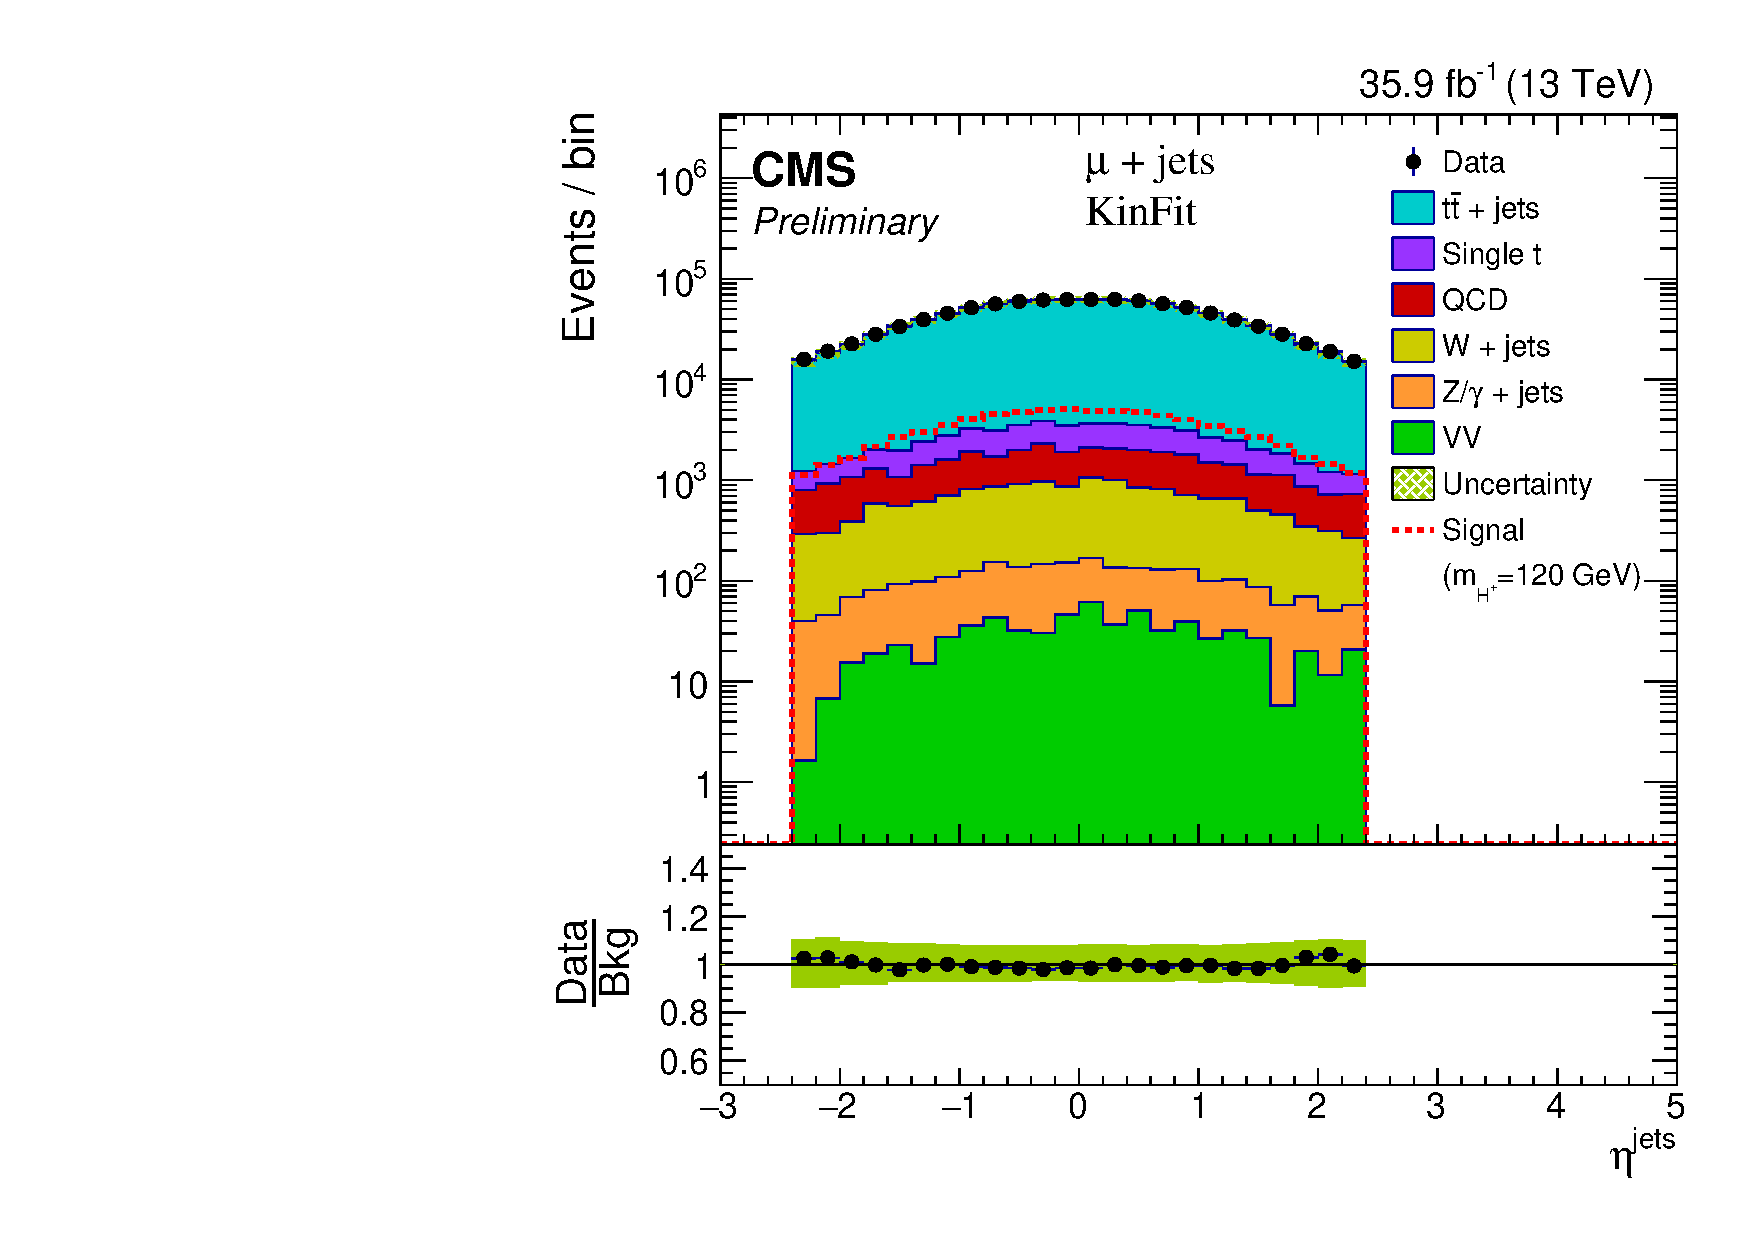
\includegraphics[width=0.40\linewidth]{Image/Muon/KinFit/eta_jet_muKinFit.pdf}}
    \subfigure[$\eta$ of jets]{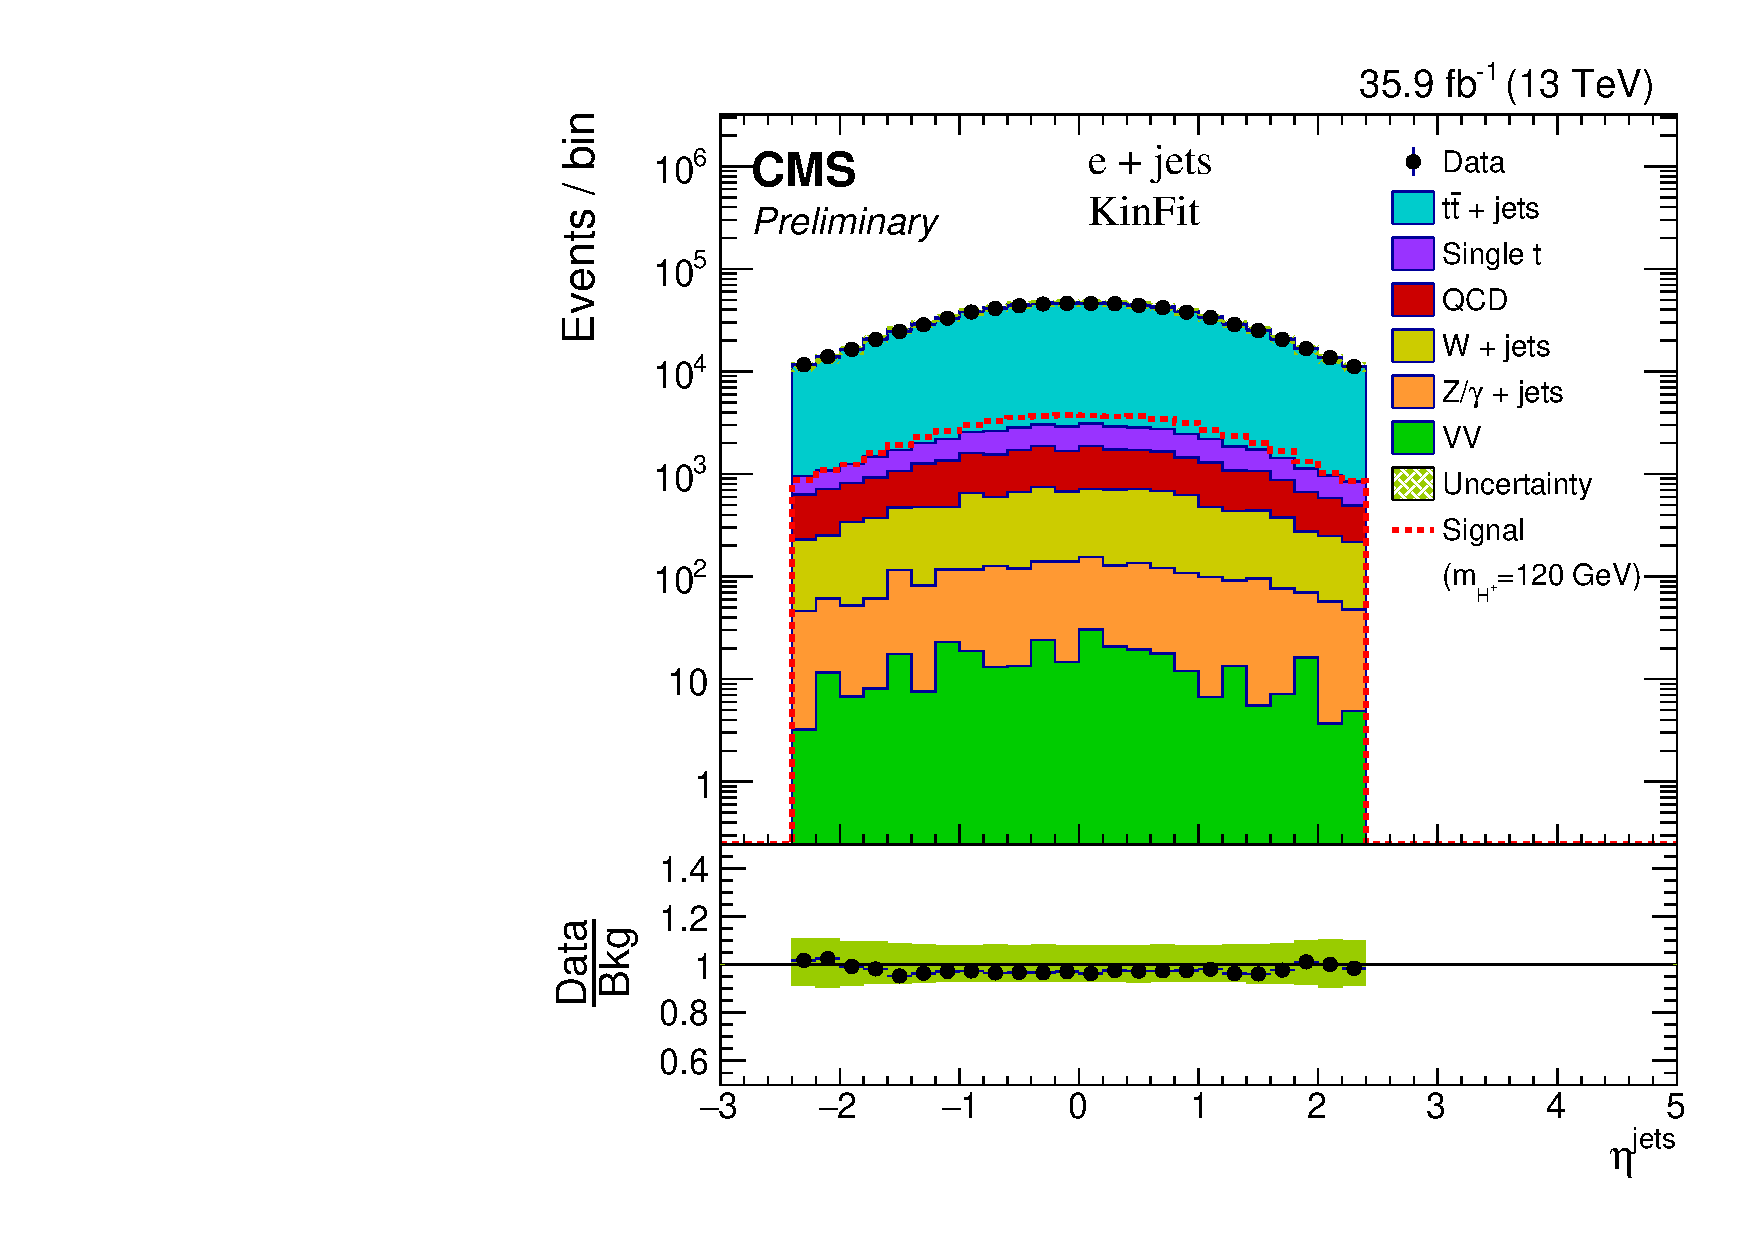
\includegraphics[width=0.40\linewidth]{Image/Electron/KinFit/eta_jet_eleKinFit.pdf}}
    \vfil
    \subfigure[jet multiplicity]{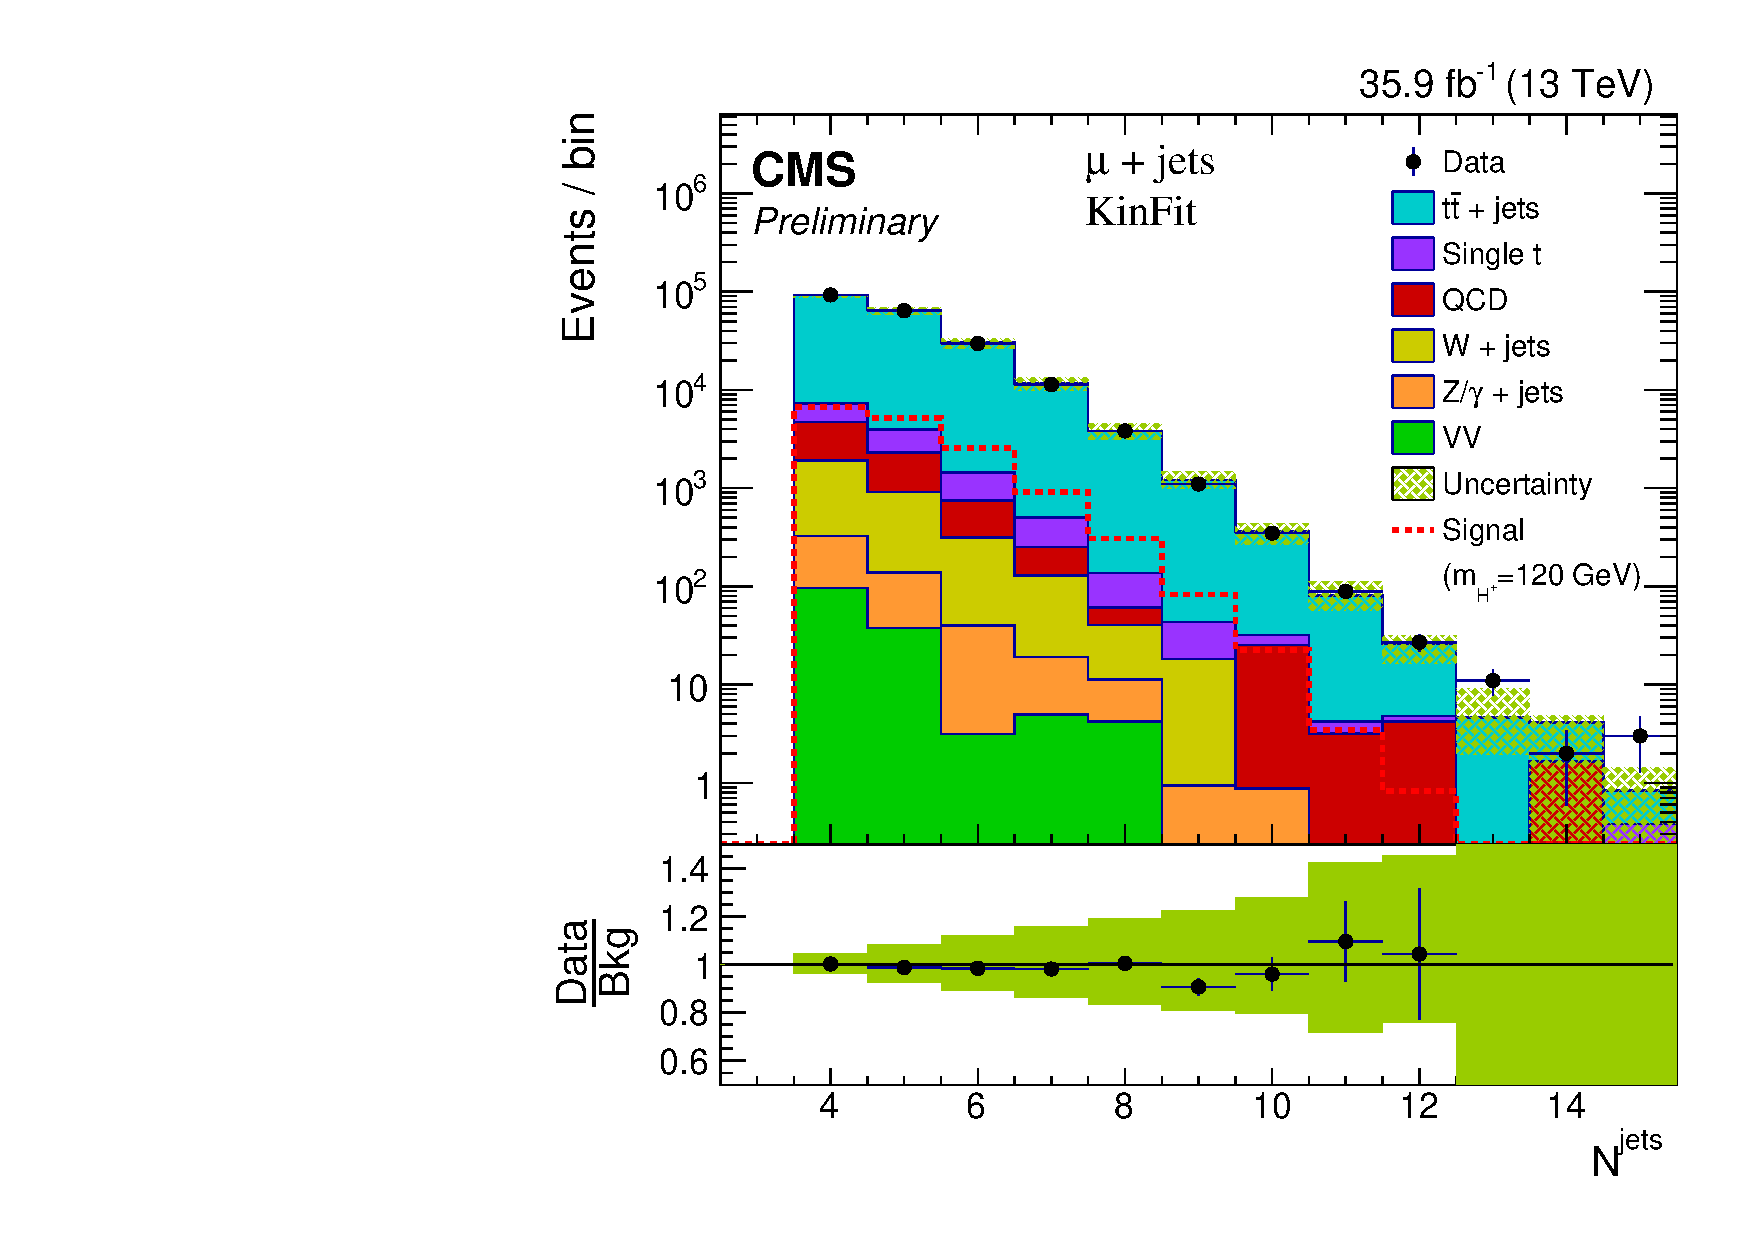
\includegraphics[width=0.40\linewidth]{Image/Muon/KinFit/final_multi_jet_muKinFit.pdf}}
    \subfigure[jet multiplicity]{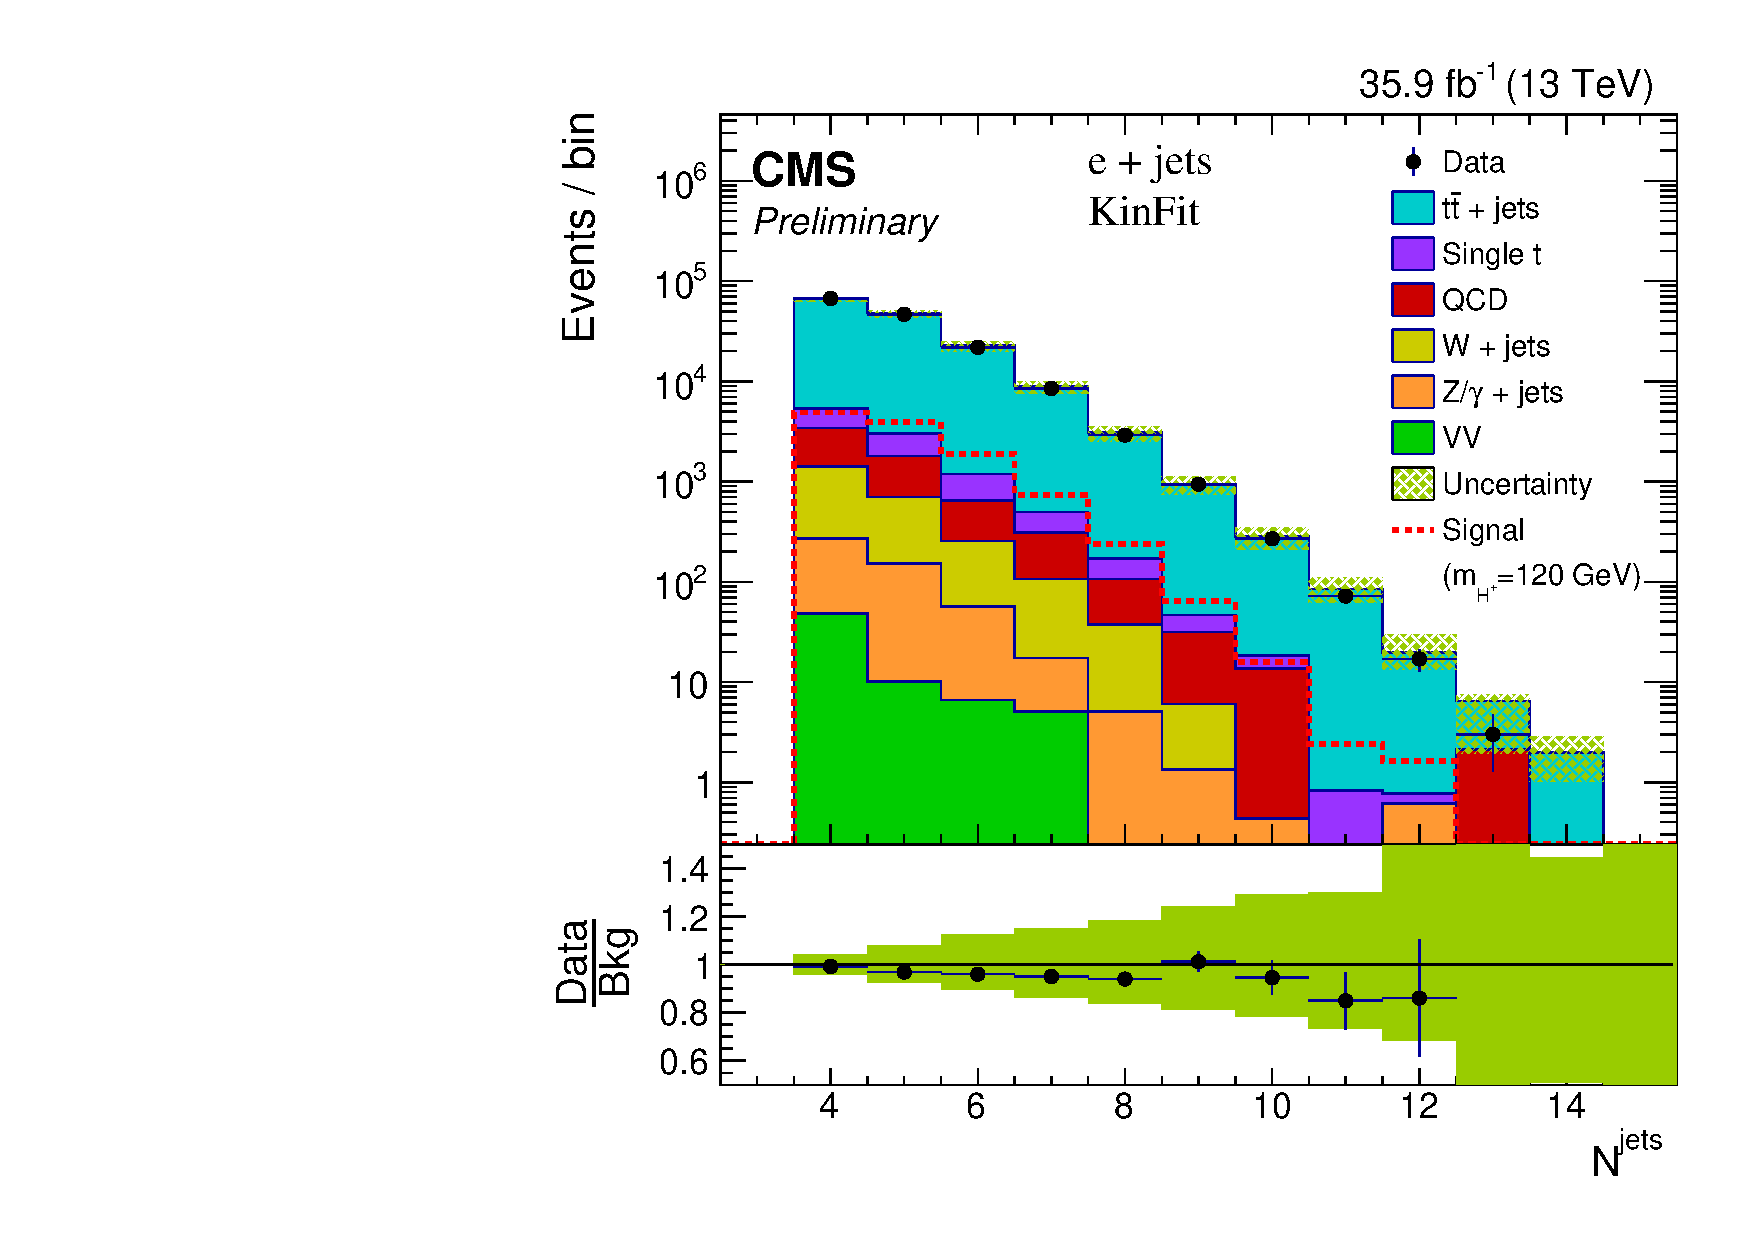
\includegraphics[width=0.40\linewidth]{Image/Electron/KinFit/final_multi_jet_eleKinFit.pdf}}
    \vfil
    \subfigure[\PQb jet multiplicity]{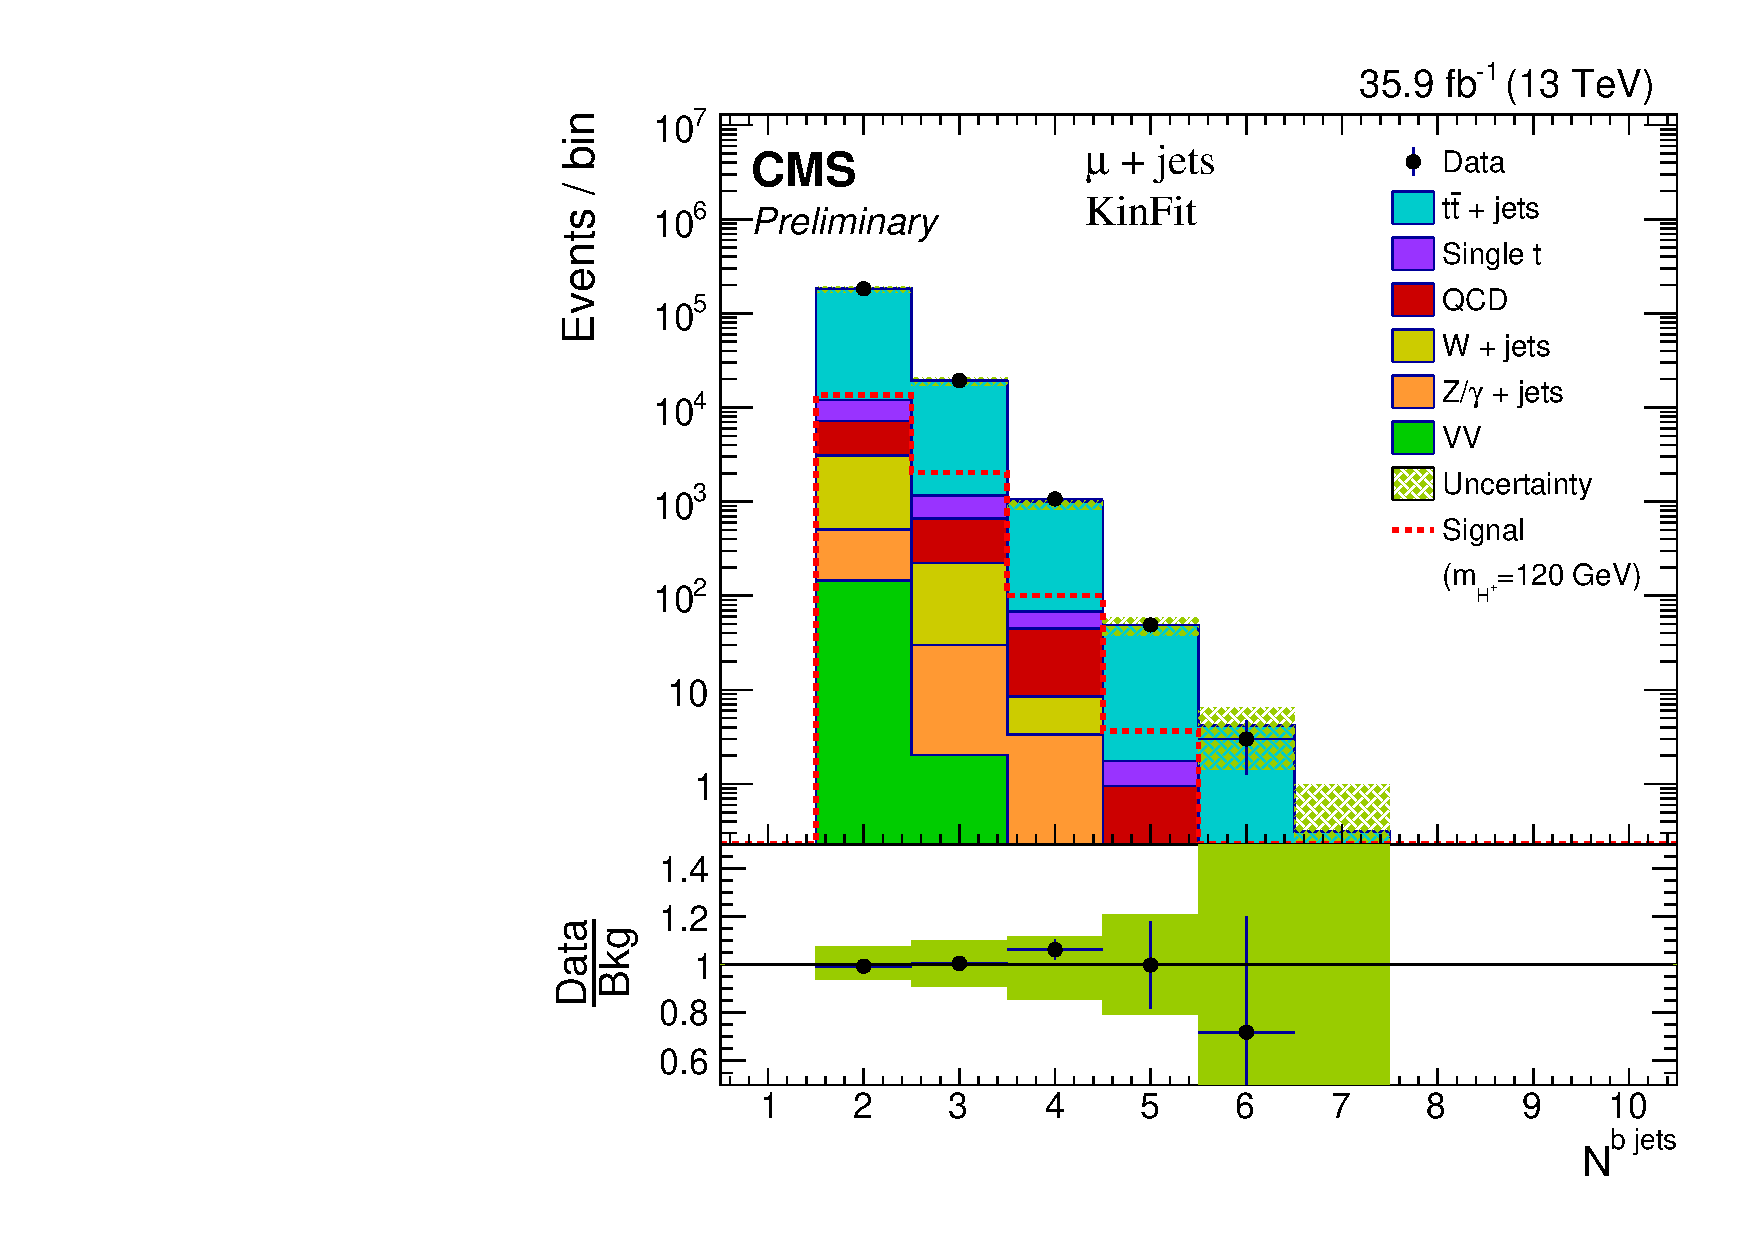
\includegraphics[width=0.40\linewidth]{Image/Muon/KinFit/CSVL_count_muKinFit.pdf}}
    \subfigure[\PQb jet multiplicity]{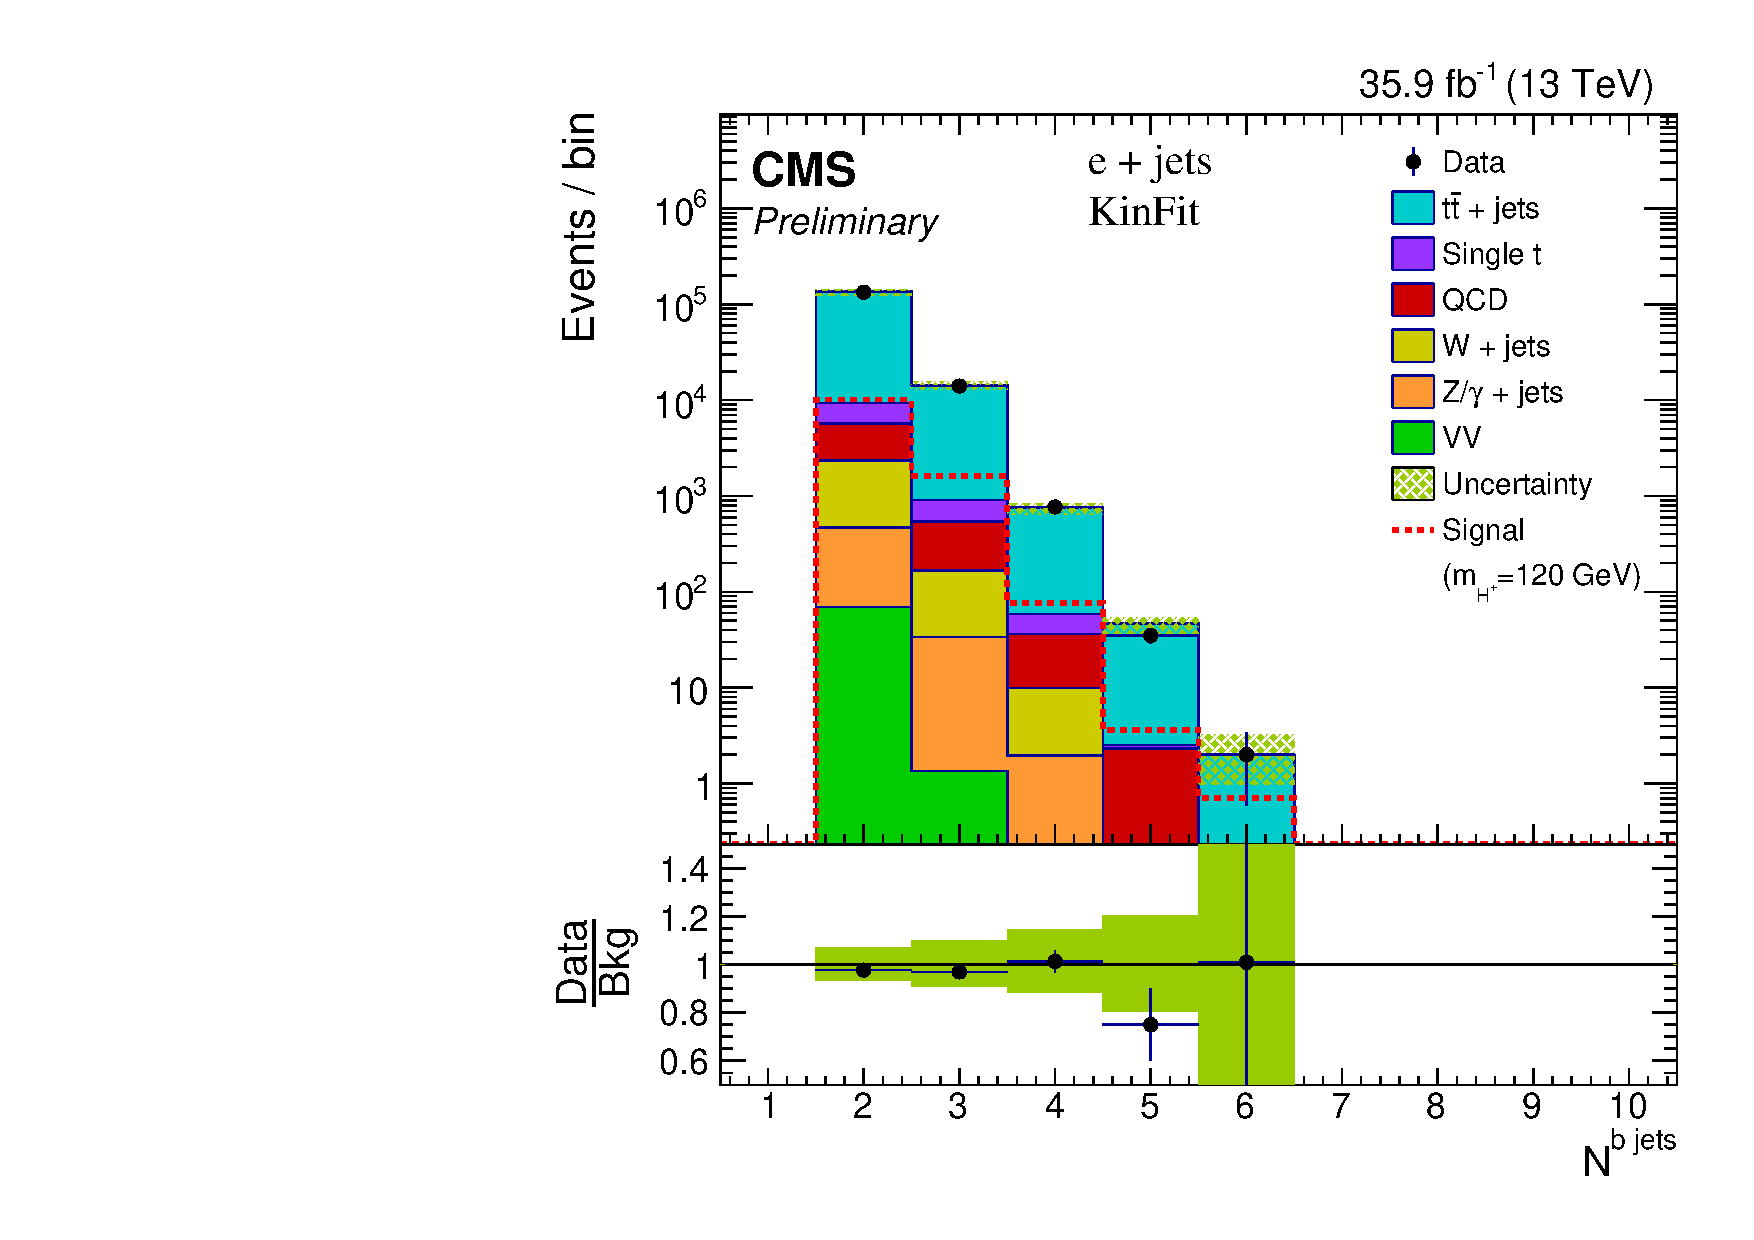
\includegraphics[width=0.40\linewidth]{Image/Electron/KinFit/CSVL_count_eleKinFit.pdf}}
    \caption{Distribution of kinematic fitted $\eta$ of jets, jet multiplicity, and \PQb jet
        multiplicity after kinematic fit selection for \mujets and \ejets channel.}
    \label{fig:kfitPlot2}
\end{figure}

\begin{figure}
    \centering  
    \subfigure[Missing transverse energy]{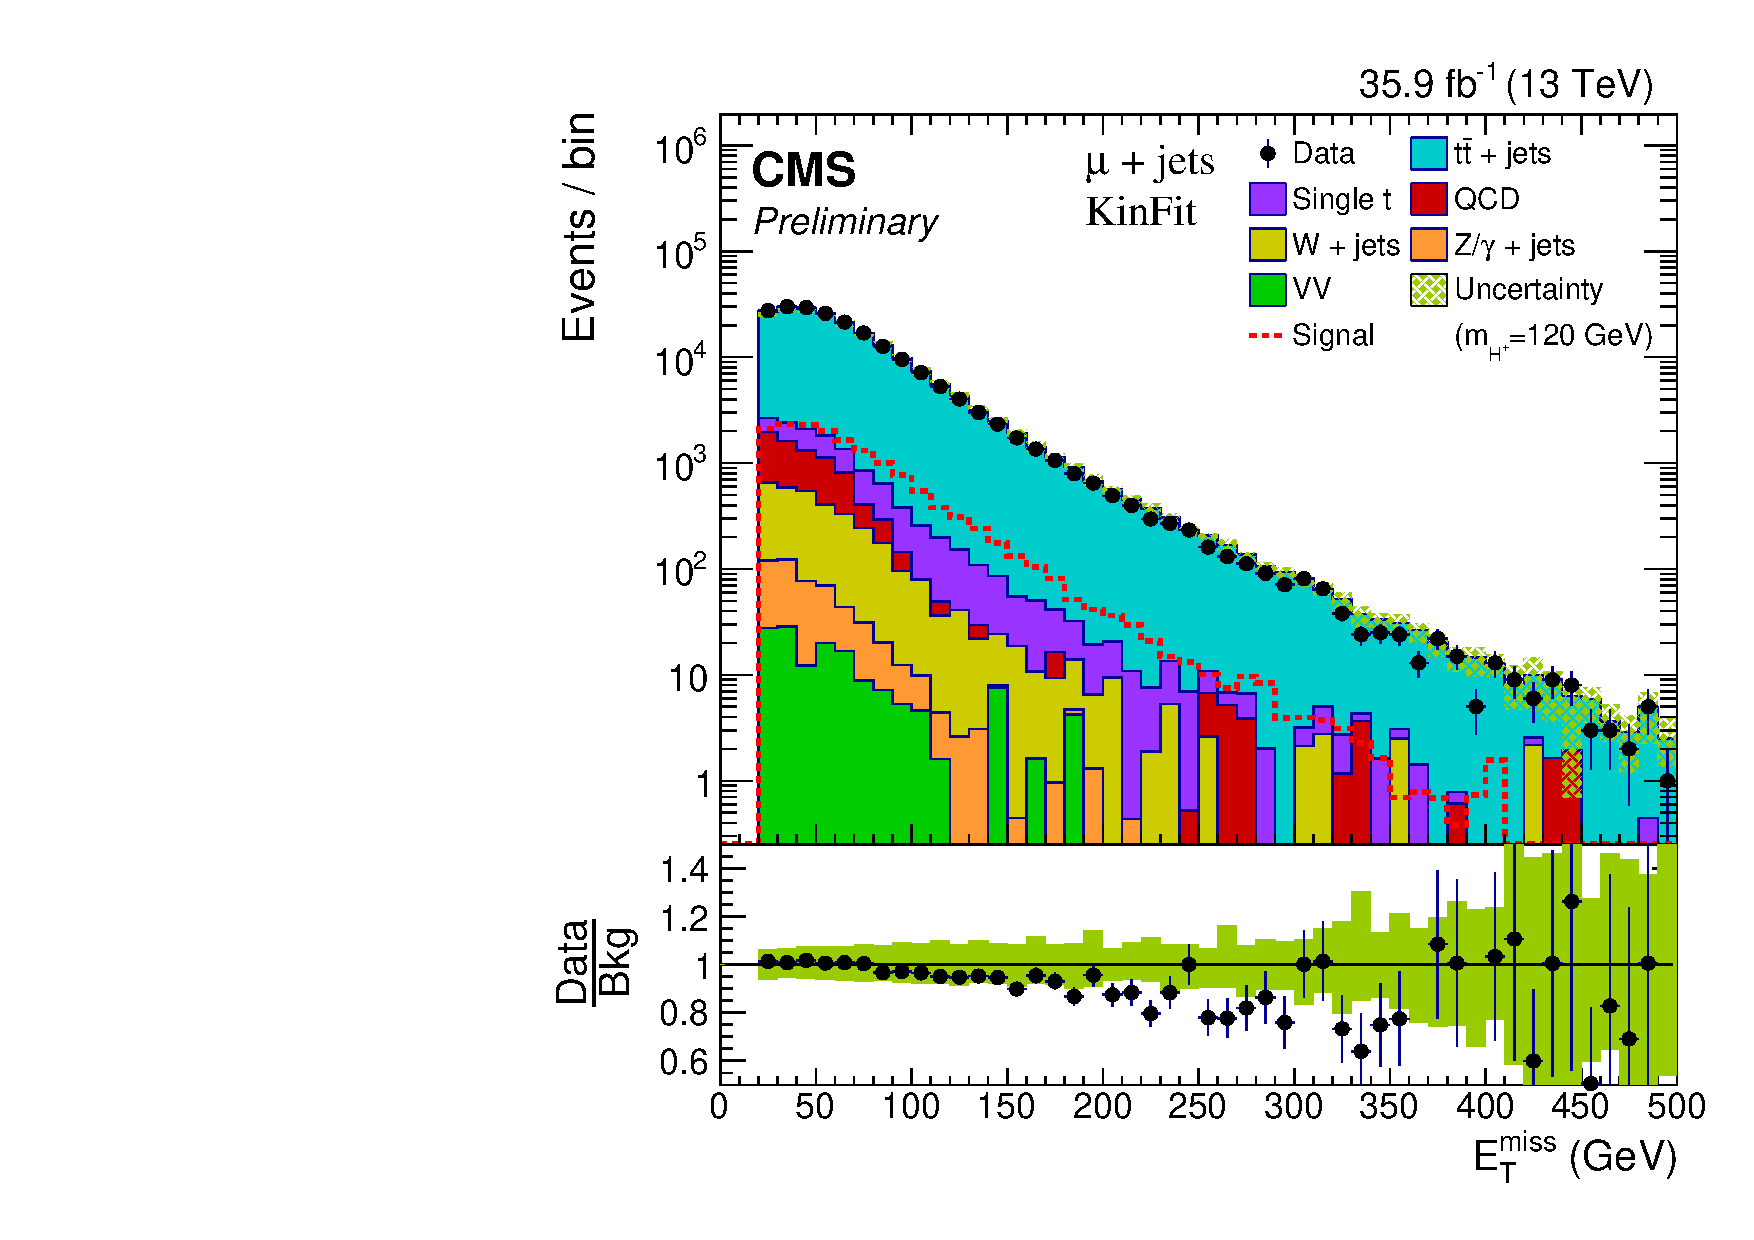
\includegraphics[width=0.45\linewidth]{Image/Muon/KinFit/final_pt_met_muKinFit.pdf}}
    \subfigure[Missing transverse energy]{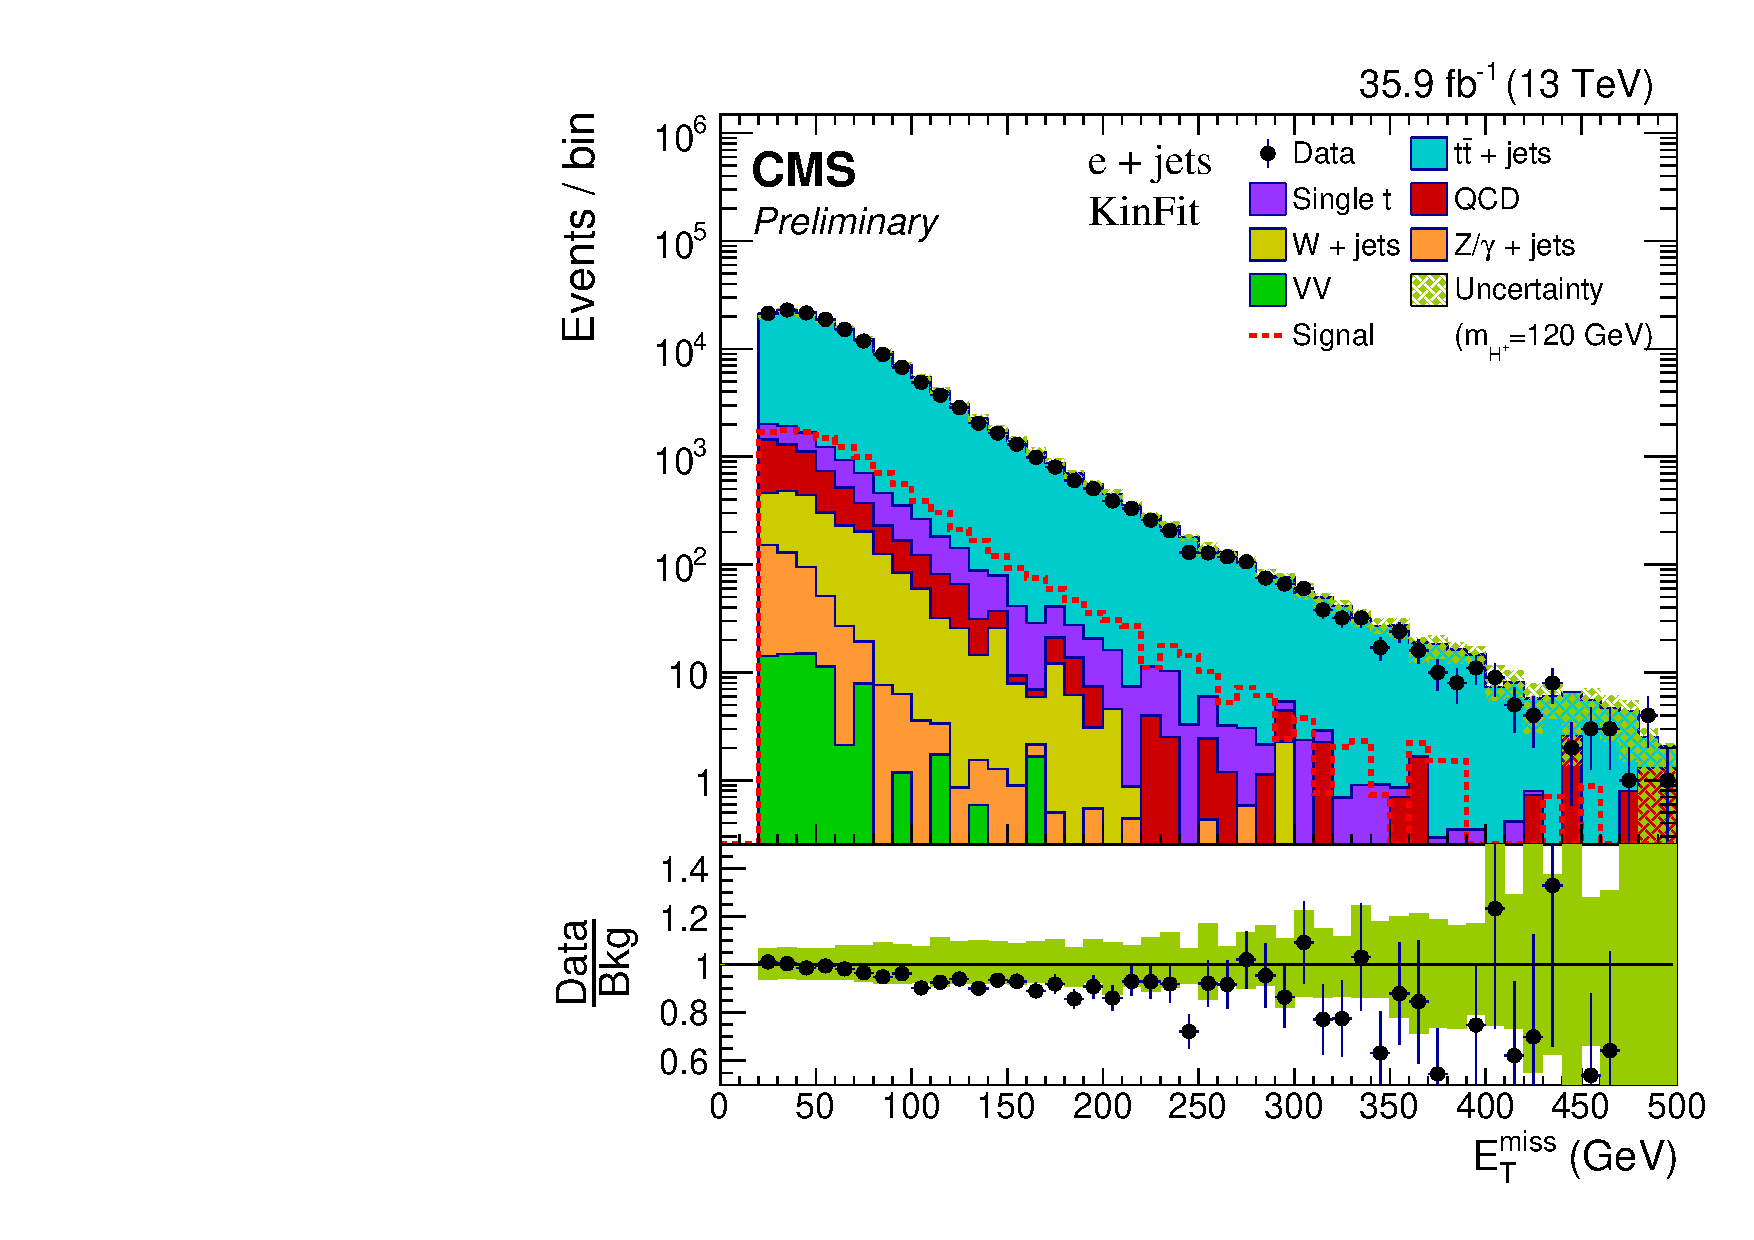
\includegraphics[width=0.45\linewidth]{Image/Electron/KinFit/final_pt_met_eleKinFit.pdf}}
    \vfil
    \subfigure[Transverse mass of \PW boson]{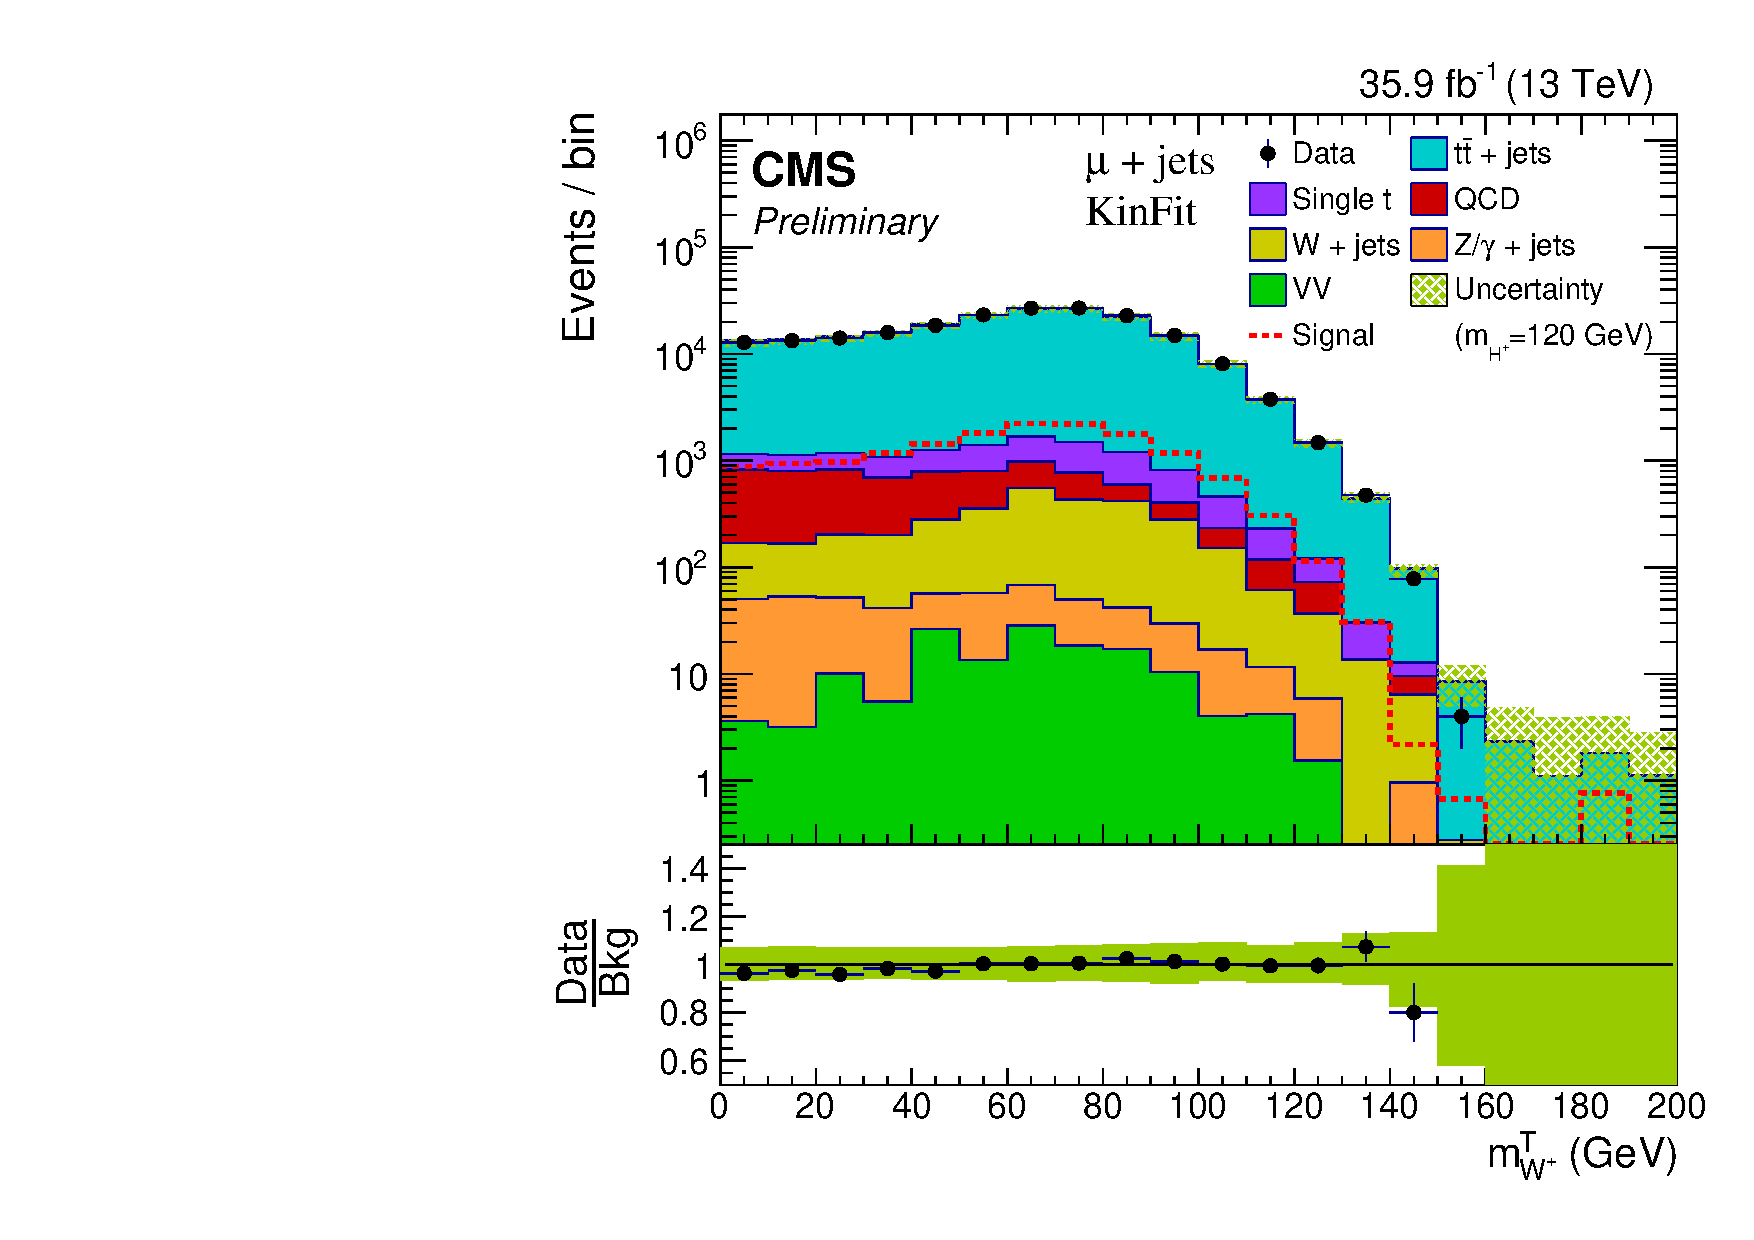
\includegraphics[width=0.45\linewidth]{Image/Muon/KinFit/wmt_muKinFit.pdf}}
    \subfigure[Transverse mass of \PW boson]{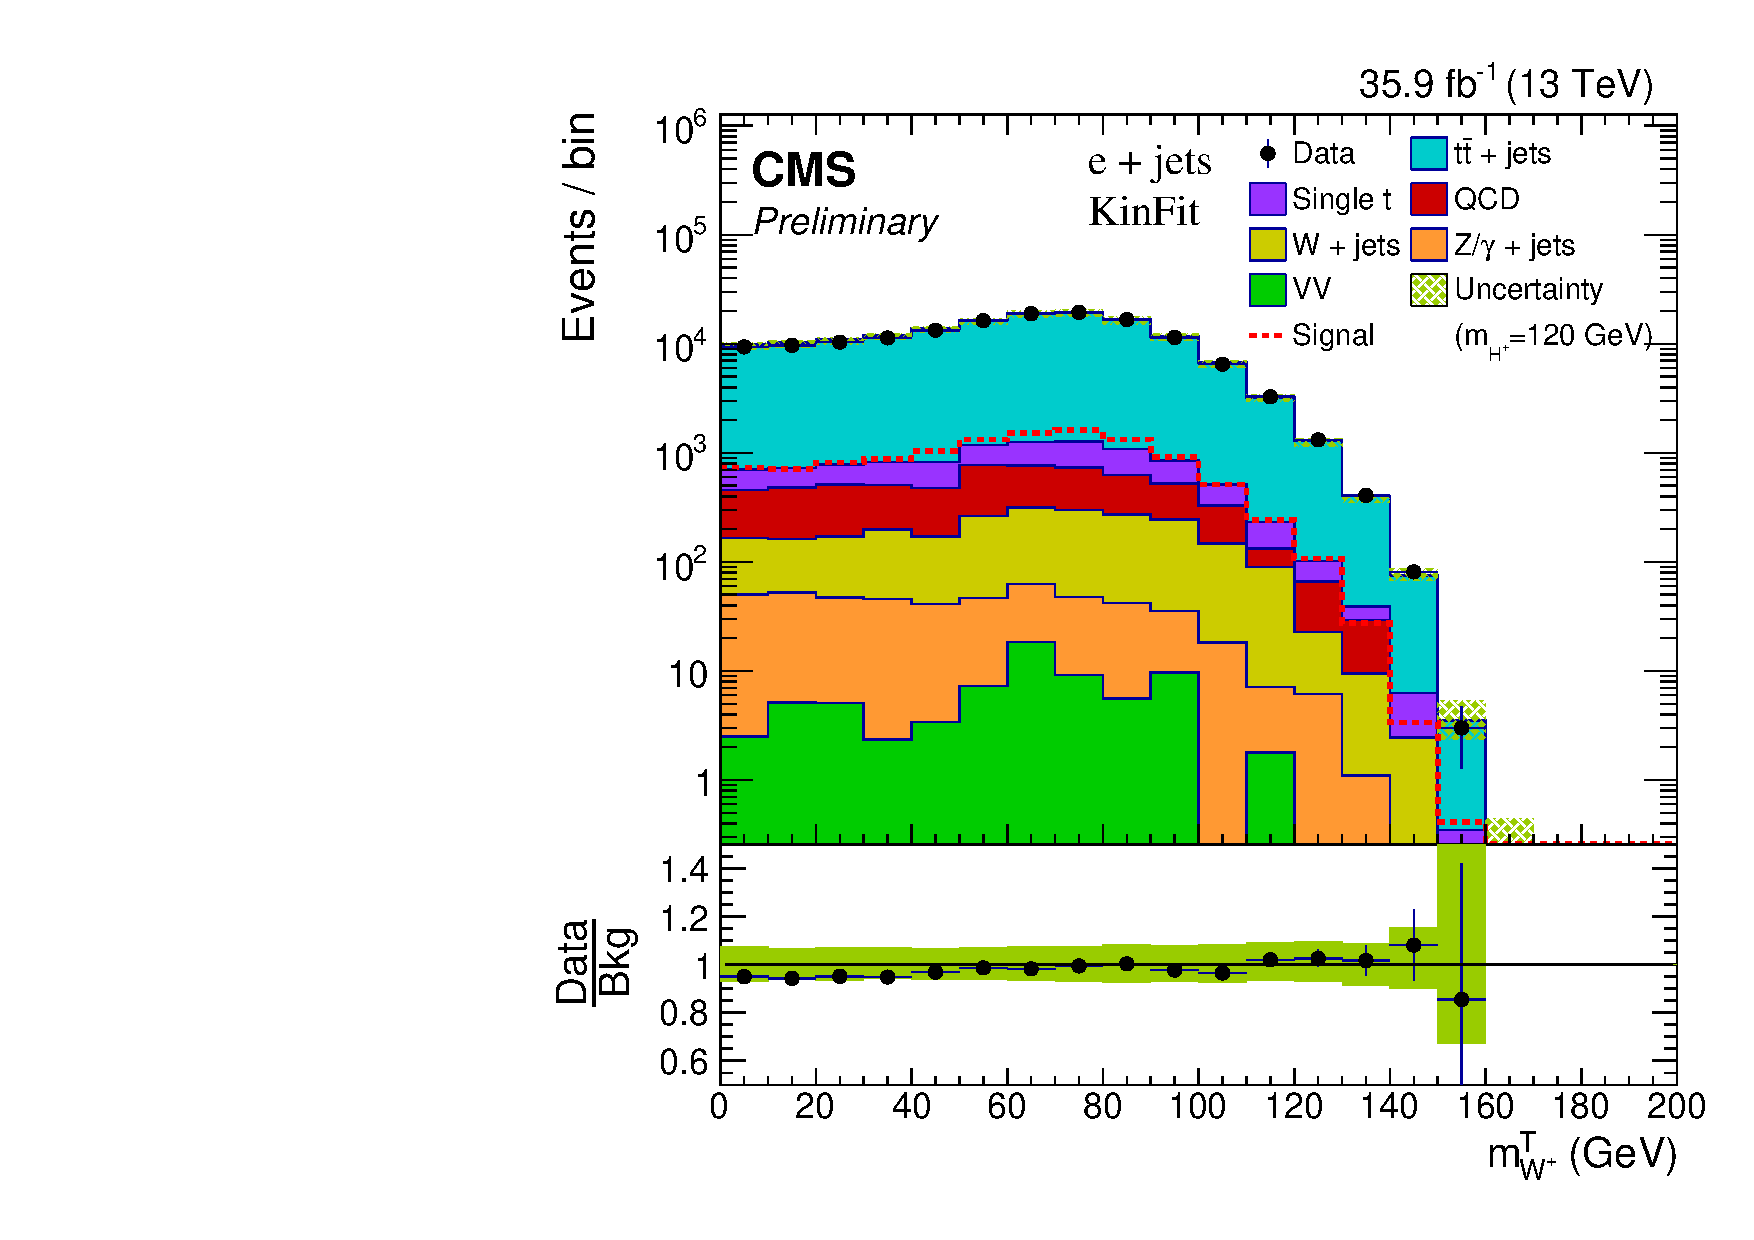
\includegraphics[width=0.45\linewidth]{Image/Electron/KinFit/wmt_eleKinFit.pdf}}
    \caption{Distribution of kinematic fitted $\MET$ and $m_{\PW^+}^{T}$ after kinematic fit selection 
	for \mujets and \ejets channel.}
    \label{fig:kfitPlot3}
\end{figure}

